\documentclass[11pt,english]{article}
\pagestyle{plain}
\pagenumbering{arabic}
\usepackage[english]{babel}
\usepackage{graphicx}
\usepackage{multirow}
\usepackage{subfig}
%\usepackage{auto-pst-pdf}
\usepackage[table,xcdraw]{xcolor}
\usepackage[T1]{fontenc}
\usepackage{hyperref}
\usepackage[hmargin={0.8cm,1.2cm},vmargin=1.2cm]{geometry}
\usepackage{lscape}
\usepackage{pdflscape}
\renewcommand*\familydefault{\sfdefault}
\newcommand{\HRule}{\rule{\linewidth}{0.5mm}}
% packages for headers and footers
\usepackage{fancyhdr}
%\usepackage{lastpage}
\pagestyle{fancy}
\fancyhf{}
%\fancyfoot[C]{Page\ \thepage\ of \pageref{LastPage}}

\begin{document}

\begin{figure}
\begin{center}
\hspace{1.5cm}
\parbox{5.5cm}{
\includegraphics[width=2.2cm]{/home/report/SCRIPTS/LOGOS/logoLaMMA}}
\hspace{.3cm}
\parbox{5.5cm}{
\includegraphics[width=2.2cm]{/home/report/SCRIPTS/LOGOS/fate_logo_11def}}
\hspace{.3cm}
\parbox{5.5cm}{
\includegraphics[width=2.2cm]{/home/report/SCRIPTS/LOGOS/logoINAFBIS}}
\hspace{.1cm}
\vspace{1.2cm}
\end{center}
\end{figure}

\begin{center}
\HRule \\[0.4cm]
%\Huge{\textbf{Progetto FATE LaMMA-OAA per ESO @ Cerro Paranal etcetcetc\ldots}}
\Huge{\textbf{Forecast system for the turbulence and meteorology at the Paranal Observatory}}
\\[0.4cm]
\LARGE{\textbf{Performance assessment - monthly report}}
\HRule \\[0.4cm]
\end{center}

\begin{center}
\vspace{2cm}\Huge{Issued: Tue, 23-05-2023\\ 10:49 Paranal local time}
\HRule \\[0.1cm]
\end{center}

%\begin{center}
%\HRule \\[0.1cm]
%\tableofcontents
%\HRule \\[0.1cm]
%\end{center}
%\newpage
\clearpage

%%%%%%%%%%%%%%%%%%%%%%%%%%%%%%%%%
\begin{figure}
\centering
\subfloat[]{\includegraphics[width=.33\linewidth,angle=-90]{/home/report/FIGS/5GG/1H/ws_sim_mnh_ar_dimm_300_960_BEF_stan.eps}}
\subfloat[]{\includegraphics[width=.33\linewidth,angle=-90]{/home/report/FIGS/5GG/1H/ws_sim_mnh_ar_dimm_300_960_AFT_stan.eps}}
\subfloat[]{\includegraphics[width=.33\linewidth,angle=-90]{/home/report/FIGS/5GG/1H/ws_sim_mnh_ar_dimm_300_960_AFT_stan_per.eps}}
\caption{\textbf{wind speed} ($m s^{-1}$): (a) STANDARD CONFIGURATION, (b) WITH AR (1H), (c) PERSISTENCE.}
\label{fig:ws}
\end{figure}
%%%%%%%%%%%%%%%%%%%%%%%%%%%%%%%%%
\begin{figure}
\centering
\subfloat[]{\includegraphics[width=.33\linewidth,angle=-90]{/home/report/FIGS/5GG/1H/wd_sim_mnh_ar_dimm_300_960_BEF_stan.eps}}
\subfloat[]{\includegraphics[width=.33\linewidth,angle=-90]{/home/report/FIGS/5GG/1H/wd_sim_mnh_ar_dimm_300_960_AFT_stan.eps}}
\subfloat[]{\includegraphics[width=.33\linewidth,angle=-90]{/home/report/FIGS/5GG/1H/wd_sim_mnh_ar_dimm_300_960_AFT_stan_per.eps}}
\caption{wind direction (degree): (a) STANDARD CONFIGURATION, (b) WITH AR, (c) PERSISTENCE.}
\label{fig:wd}
\end{figure}
%%%%%%%%%%%%%%%%%%%%%%%%%%%%%%%%%
\begin{figure}
\centering
\subfloat[]{\includegraphics[width=.33\linewidth,angle=-90]{/home/report/FIGS/5GG/1H/rh_sim_mnh_ar_dimm_300_960_BEF_stan.eps}}
\subfloat[]{\includegraphics[width=.33\linewidth,angle=-90]{/home/report/FIGS/5GG/1H/rh_sim_mnh_ar_dimm_300_960_AFT_stan.eps}}
\subfloat[]{\includegraphics[width=.33\linewidth,angle=-90]{/home/report/FIGS/5GG/1H/rh_sim_mnh_ar_dimm_300_960_AFT_stan_per.eps}}
\caption{relative humidity (percent): (a) STANDARD CONFIGURATION, (b) WITH AR (1H), (c) PERSISTENCE.}
\label{fig:rh}
\end{figure}
%%%%%%%%%%%%%%%%%%%%%%%%%%%%%%%%%
\begin{figure}
\centering
\subfloat[]{\includegraphics[width=.33\linewidth,angle=-90]{/home/report/FIGS/5GG/1H/pwv_sim_mnh_ar_dimm_300_960_BEF_stan.eps}}
\subfloat[]{\includegraphics[width=.33\linewidth,angle=-90]{/home/report/FIGS/5GG/1H/pwv_sim_mnh_ar_dimm_300_960_AFT_stan.eps}}
\subfloat[]{\includegraphics[width=.33\linewidth,angle=-90]{/home/report/FIGS/5GG/1H/pwv_sim_mnh_ar_dimm_300_960_AFT_stan_per.eps}}
\caption{precipitable water vapor (mm): (a) STANDARD CONFIGURATION, (b) WITH AR (1H), (c) PERSISTENCE.}
\label{fig:pwv}
\end{figure}
%%%%%%%%%%%%%%%%%%%%%%%%%%%%%%%%%
\begin{figure}
\centering
\subfloat[]{\includegraphics[width=.33\linewidth,angle=-90]{/home/report/FIGS/5GG/1H/see_sim_mnh_ar_dimm_300_960_BEF_os18_1000.eps}}
\subfloat[]{\includegraphics[width=.33\linewidth,angle=-90]{/home/report/FIGS/5GG/1H/see_sim_mnh_ar_dimm_300_960_AFT_os18_1000.eps}}
\subfloat[]{\includegraphics[width=.33\linewidth,angle=-90]{/home/report/FIGS/5GG/1H/see_sim_mnh_ar_dimm_300_960_AFT_os18_1000_per.eps}}
\caption{total seeing (arcsec): (a) STANDARD CONFIGURATION ($<$ 1.5''), (b) WITH AR (1H), (c) PERSISTENCE.}
\label{fig:see}
\end{figure}
%%%%%%%%%%%%%%%%%%%%%%%%%%%%%%%%%
\begin{figure}
\centering
\subfloat[]{\includegraphics[width=.33\linewidth,angle=-90]{/home/report/FIGS/5GG/1H/tau_sim_mnh_ar_dimm_300_960_BEF_os18_1000.eps}}
\subfloat[]{\includegraphics[width=.33\linewidth,angle=-90]{/home/report/FIGS/5GG/1H/tau_sim_mnh_ar_dimm_300_960_AFT_os18_1000.eps}}
\subfloat[]{\includegraphics[width=.33\linewidth,angle=-90]{/home/report/FIGS/5GG/1H/tau_sim_mnh_ar_dimm_300_960_AFT_os18_1000_per.eps}}
\caption{coeherence time (ms): (a) STANDARD CONFIGURATION, (b) WITH AR (1H), (c) PERSISTENCE.}
\label{fig:tau}
\end{figure}
%%%%%%%%%%%%%%%%%%%%%%%%%%%%%%%%%
\begin{figure}
\centering
\subfloat[]{\includegraphics[width=.33\linewidth,angle=-90]{/home/report/FIGS/5GG/1H/glf_sim_mnh_ar_dimm_300_960_BEF_os18.eps}}
\subfloat[]{\includegraphics[width=.33\linewidth,angle=-90]{/home/report/FIGS/5GG/1H/glf_sim_mnh_ar_dimm_300_960_AFT_os18.eps}}
\subfloat[]{\includegraphics[width=.33\linewidth,angle=-90]{/home/report/FIGS/5GG/1H/glf_sim_mnh_ar_dimm_300_960_AFT_os18_per.eps}}
\caption{ground layer fraction (dimensionless): (a) STANDARD CONFIGURATION, (b) WITH AR (1H), (c) PERSISTENCE.}
\label{fig:glf}
\end{figure}
%%%%%%%%%%%%%%%%%%%%%%%%%%%%%%%%%
\begin{figure}
\centering
\subfloat[]{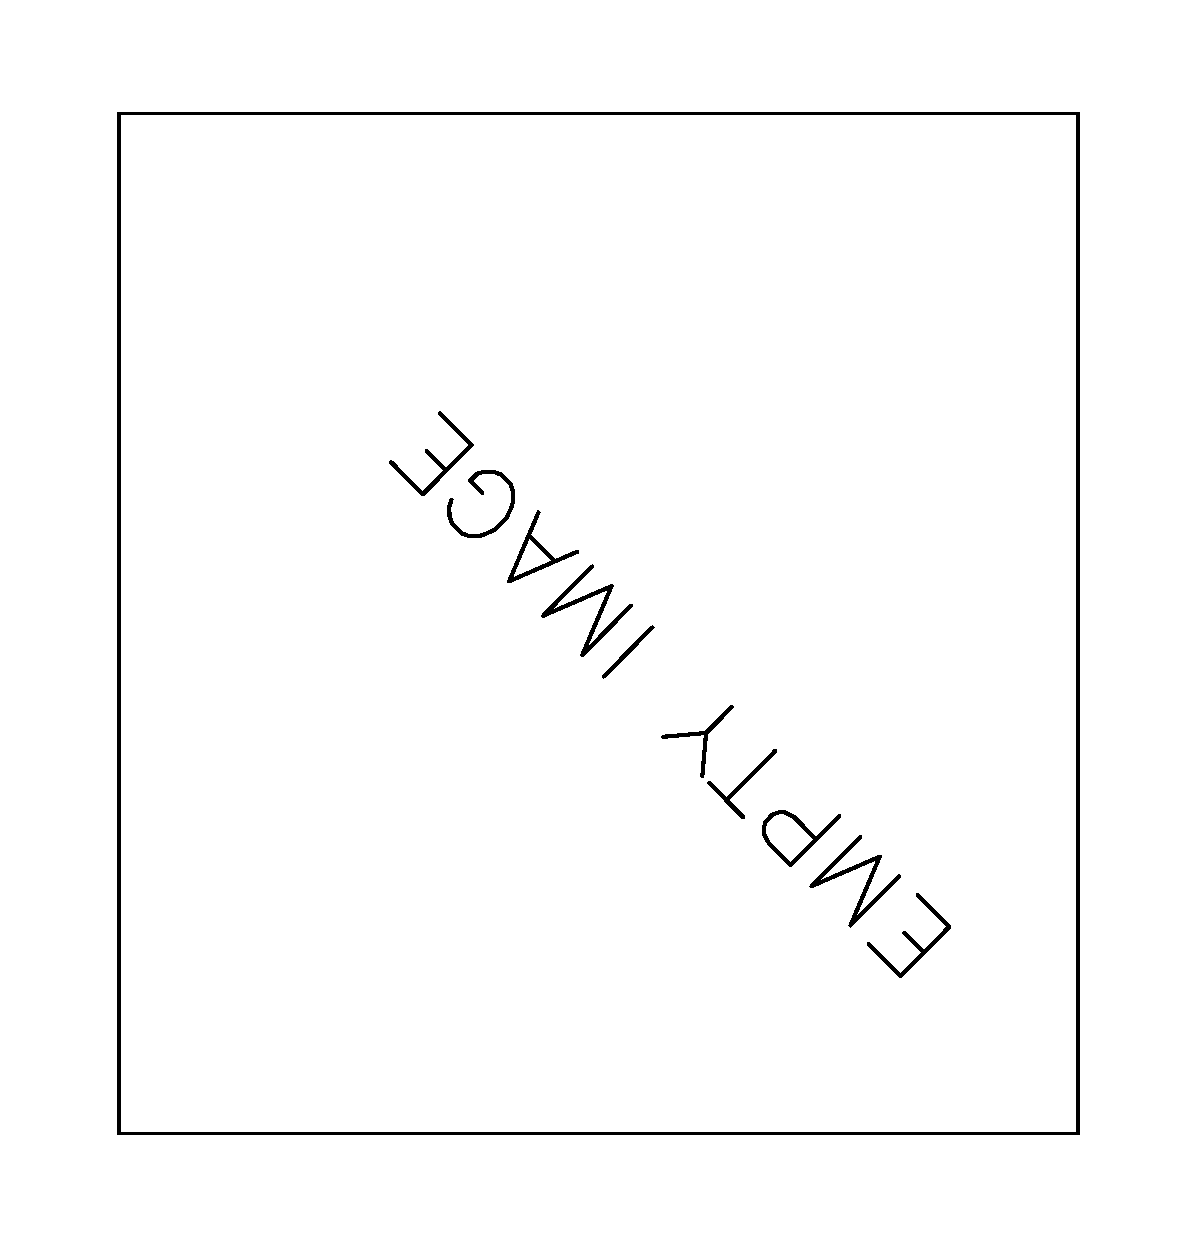
\includegraphics[width=.27\linewidth,angle=-90]{/home/report/FIGS/5GG/1H/emptyimg}}
\subfloat[]{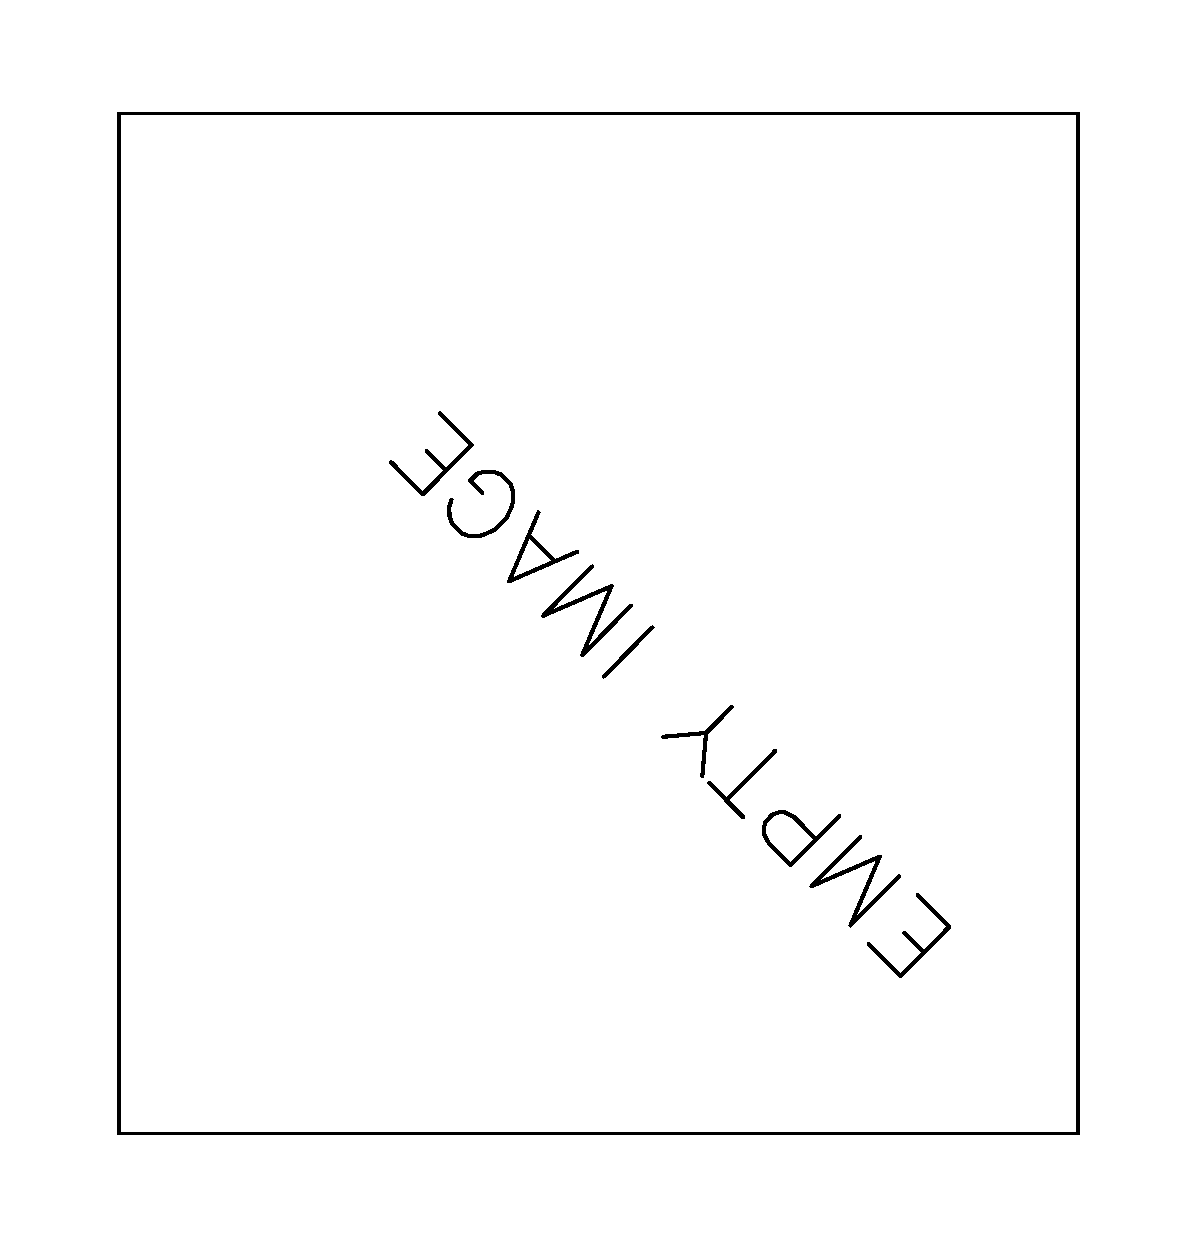
\includegraphics[width=.27\linewidth,angle=-90]{/home/report/FIGS/5GG/1H/emptyimg}}
\subfloat[]{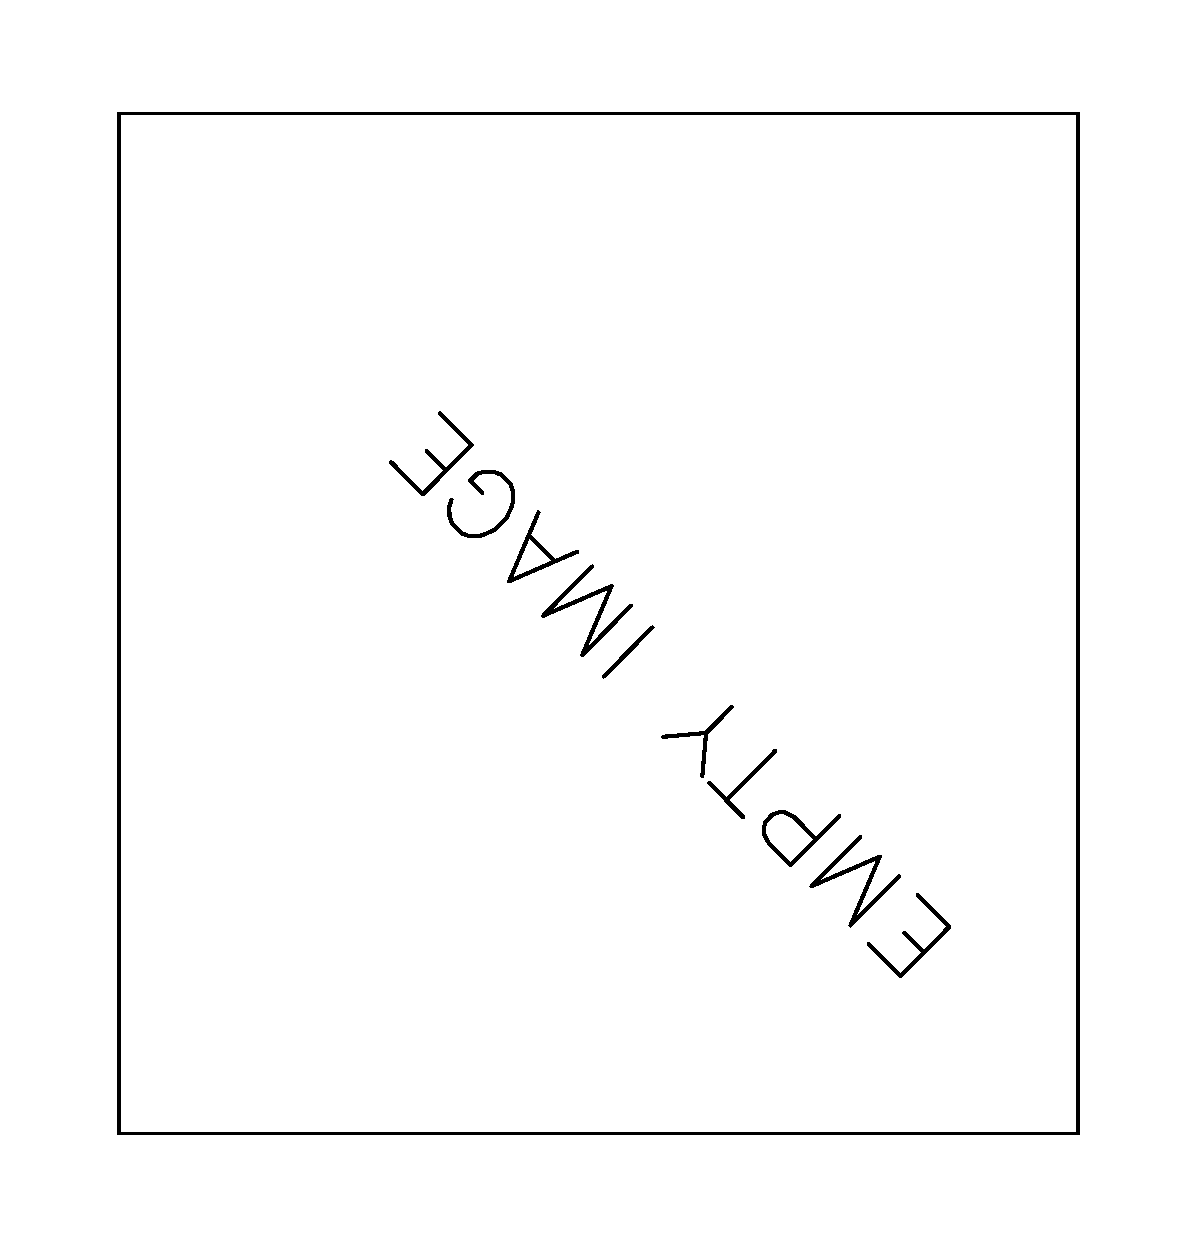
\includegraphics[width=.27\linewidth,angle=-90]{/home/report/FIGS/5GG/1H/emptyimg}}
\caption{TEST-TEST-TEST: (a) STANDARD CONFIGURATION, (b) WITH AR, (c) PERSISTENCE.}
\label{fig:ws}
\end{figure}
%%%%%%%%%%%%%%%%%%%%%%%%%%%%%%%%%
\begin{figure}
\centering
\subfloat[]{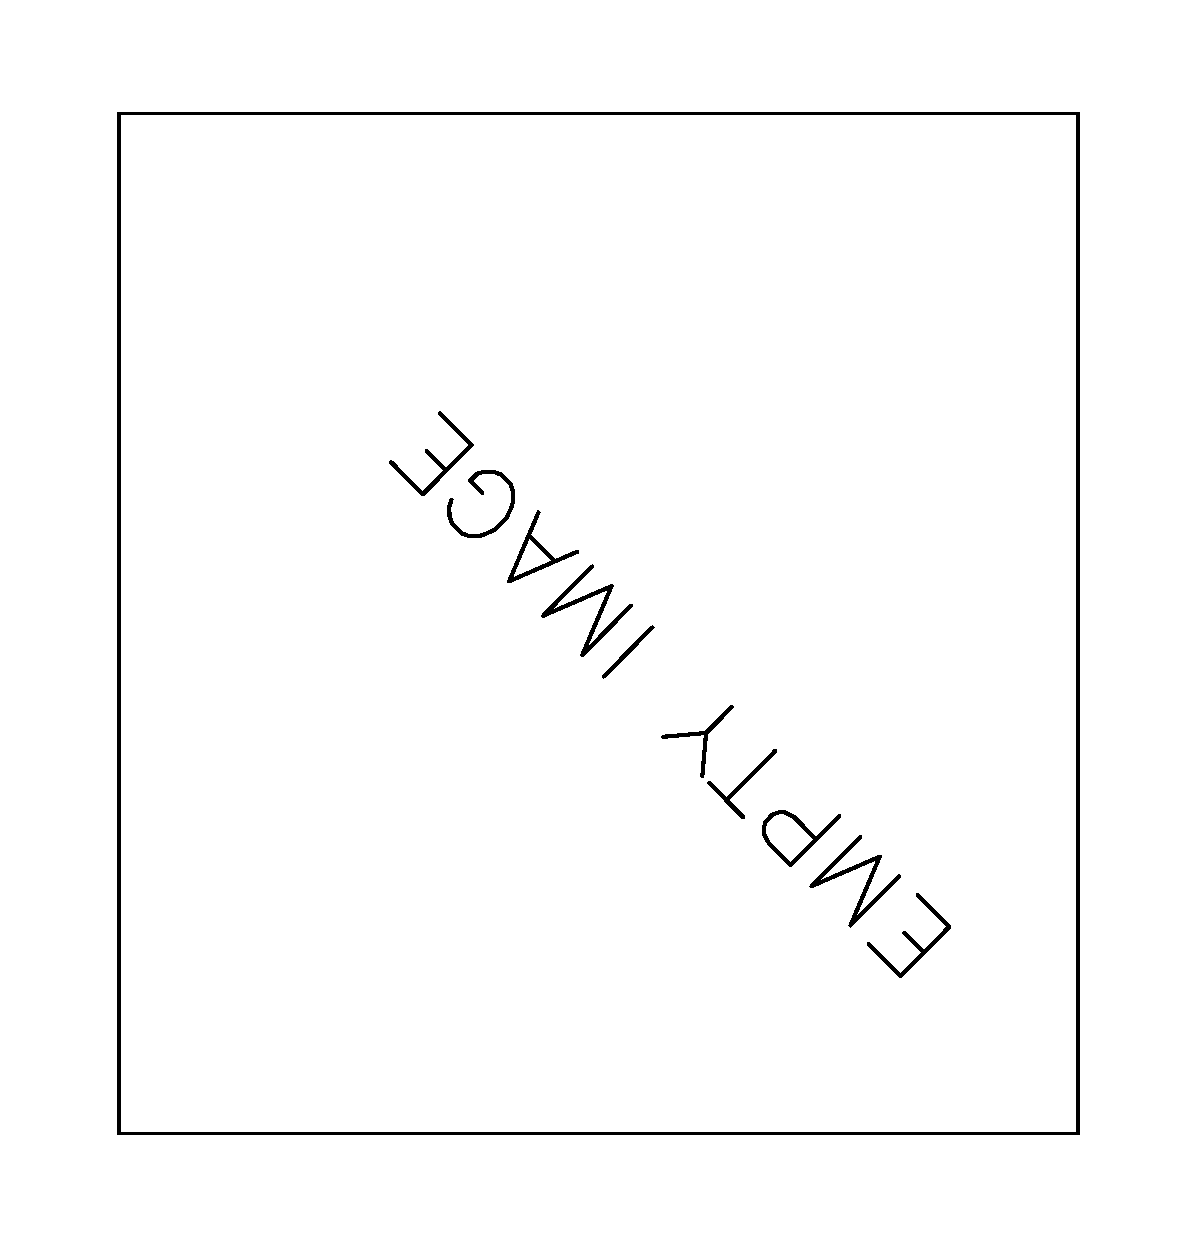
\includegraphics[width=.27\linewidth,angle=-90]{/home/report/FIGS/5GG/1H/emptyimg}}
\subfloat[]{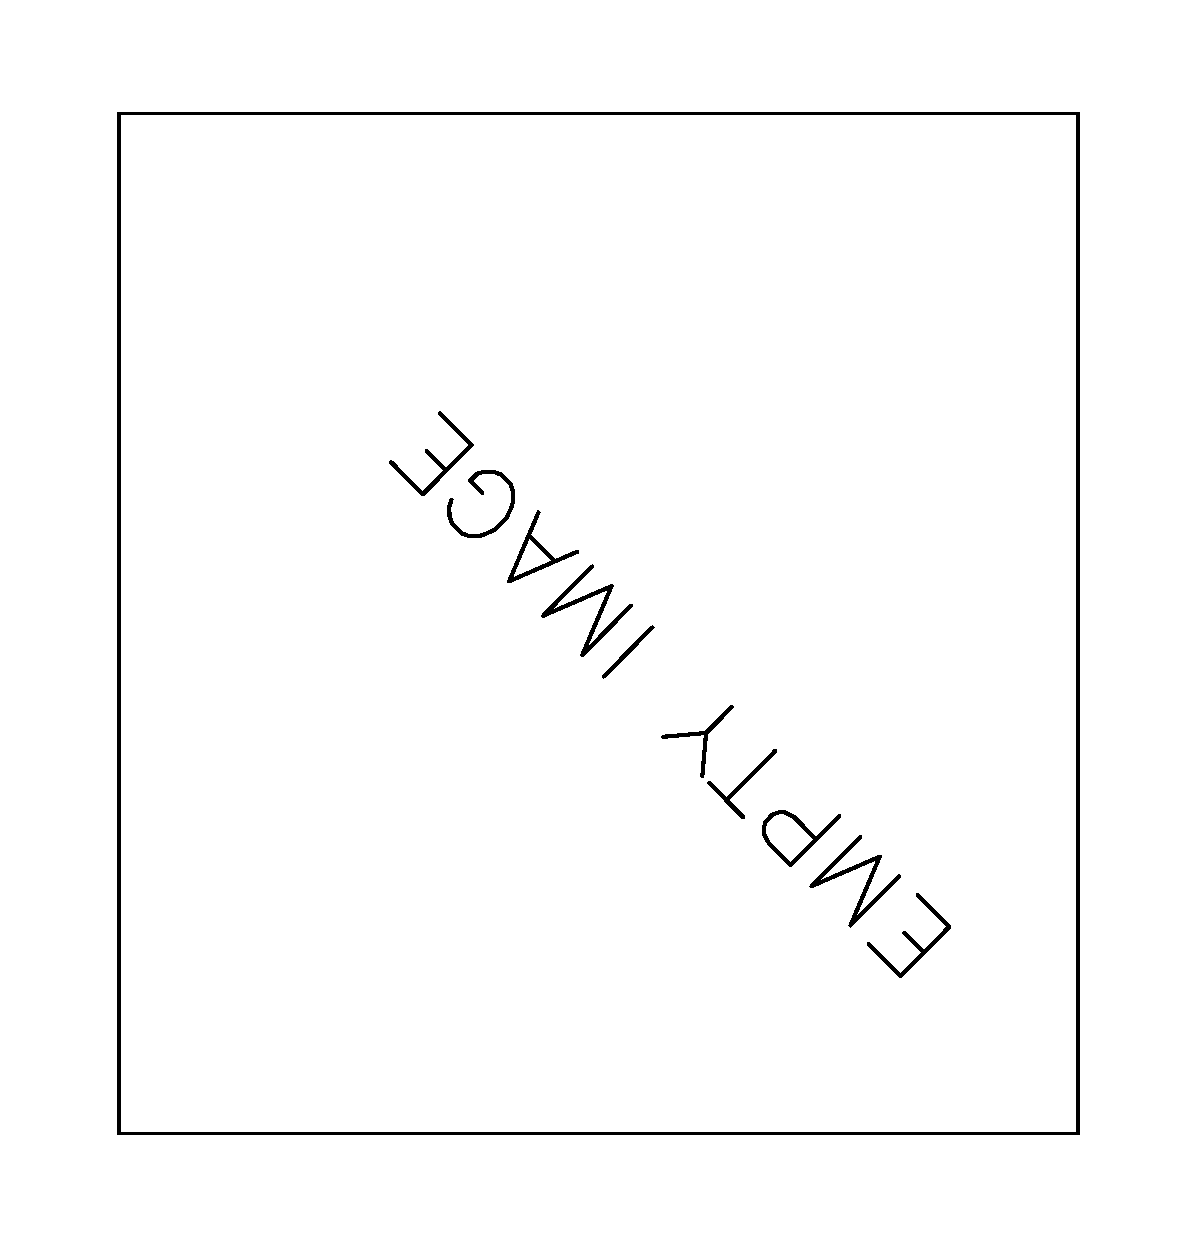
\includegraphics[width=.27\linewidth,angle=-90]{/home/report/FIGS/5GG/1H/emptyimg}}
\subfloat[]{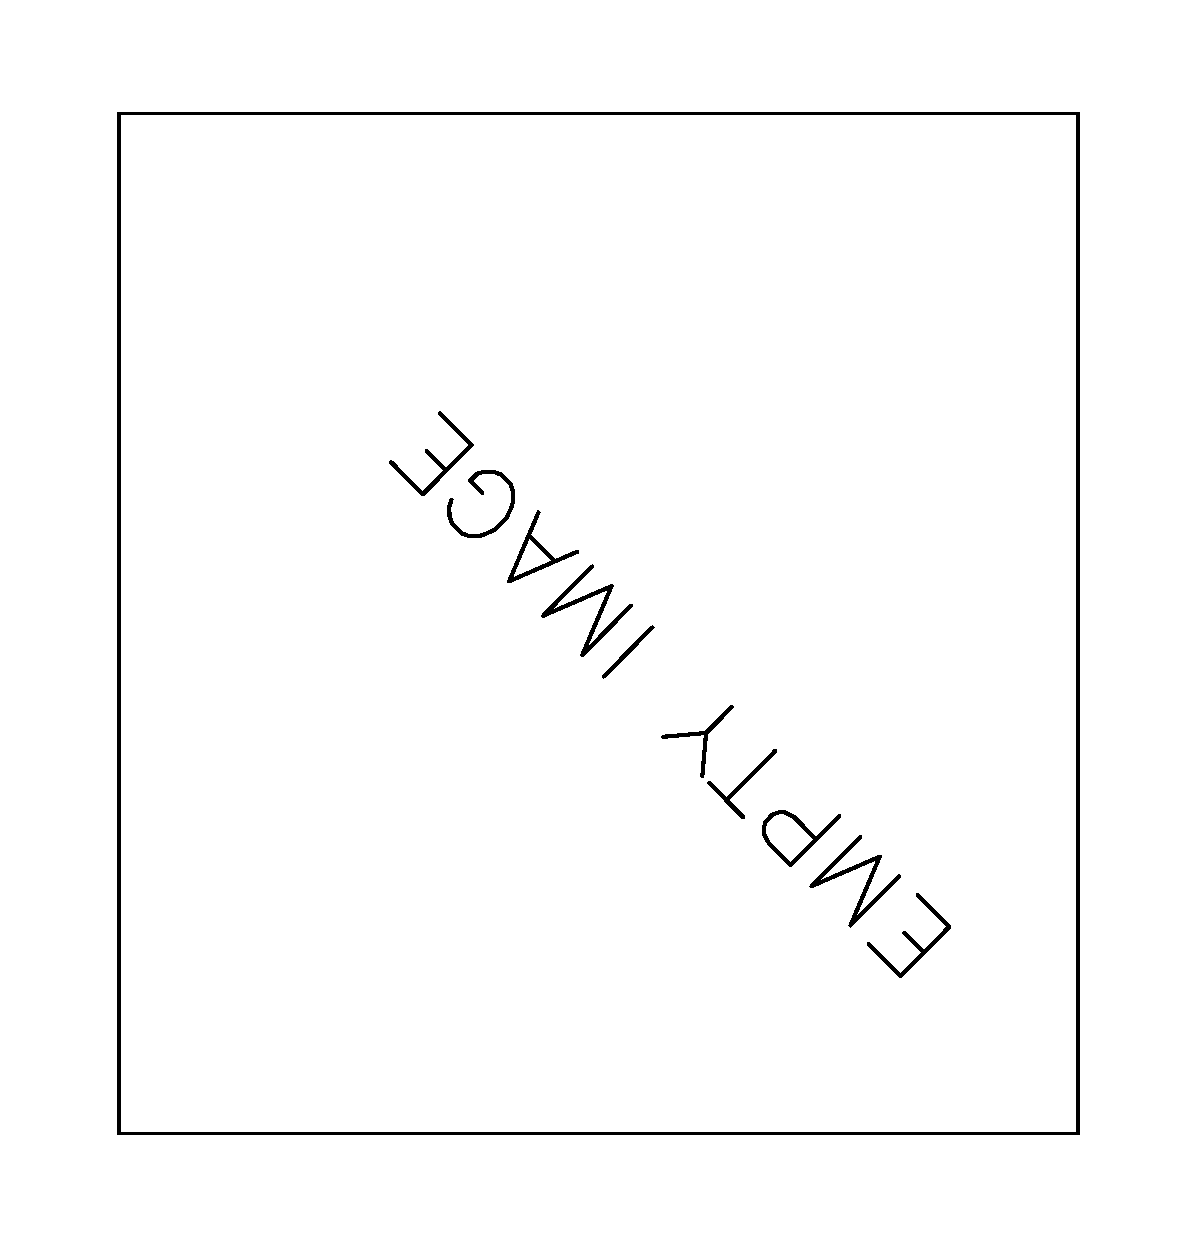
\includegraphics[width=.27\linewidth,angle=-90]{/home/report/FIGS/5GG/1H/emptyimg}}
\caption{TEST-TEST-TEST: (a) STANDARD CONFIGURATION, (b) WITH AR, (c) PERSISTENCE.}
\label{fig:ws}
\end{figure}
%%%%%%%%%%%%%%%%%%%%%%%%%%%%%%%%%
\begin{figure}
\centering
\subfloat[]{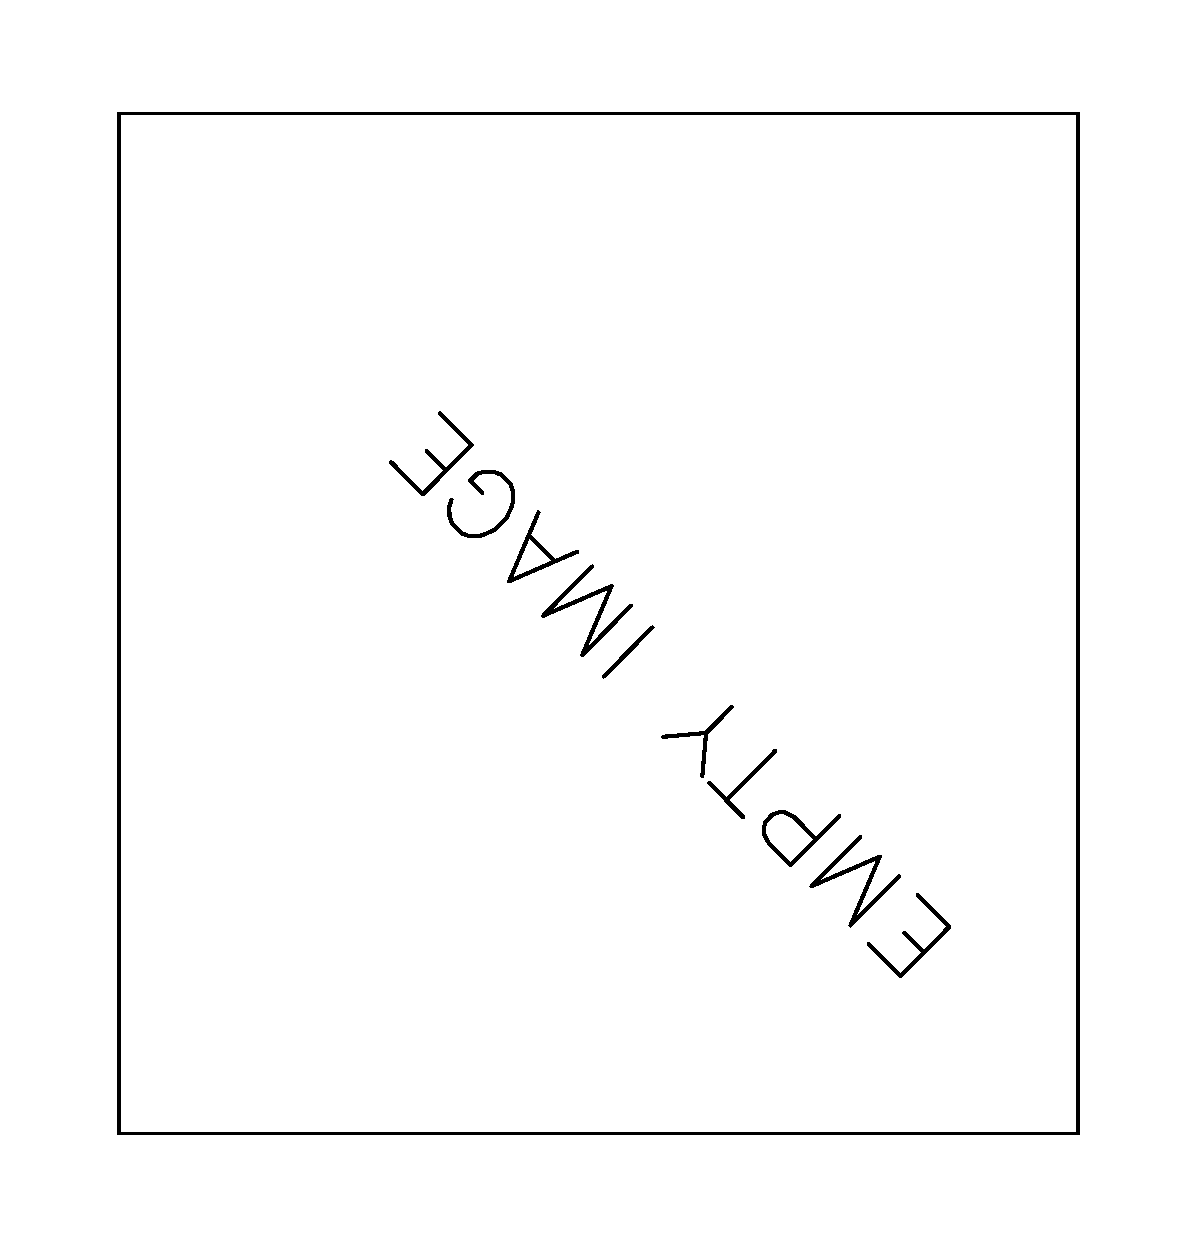
\includegraphics[width=.27\linewidth,angle=-90]{/home/report/FIGS/5GG/1H/emptyimg}}
\subfloat[]{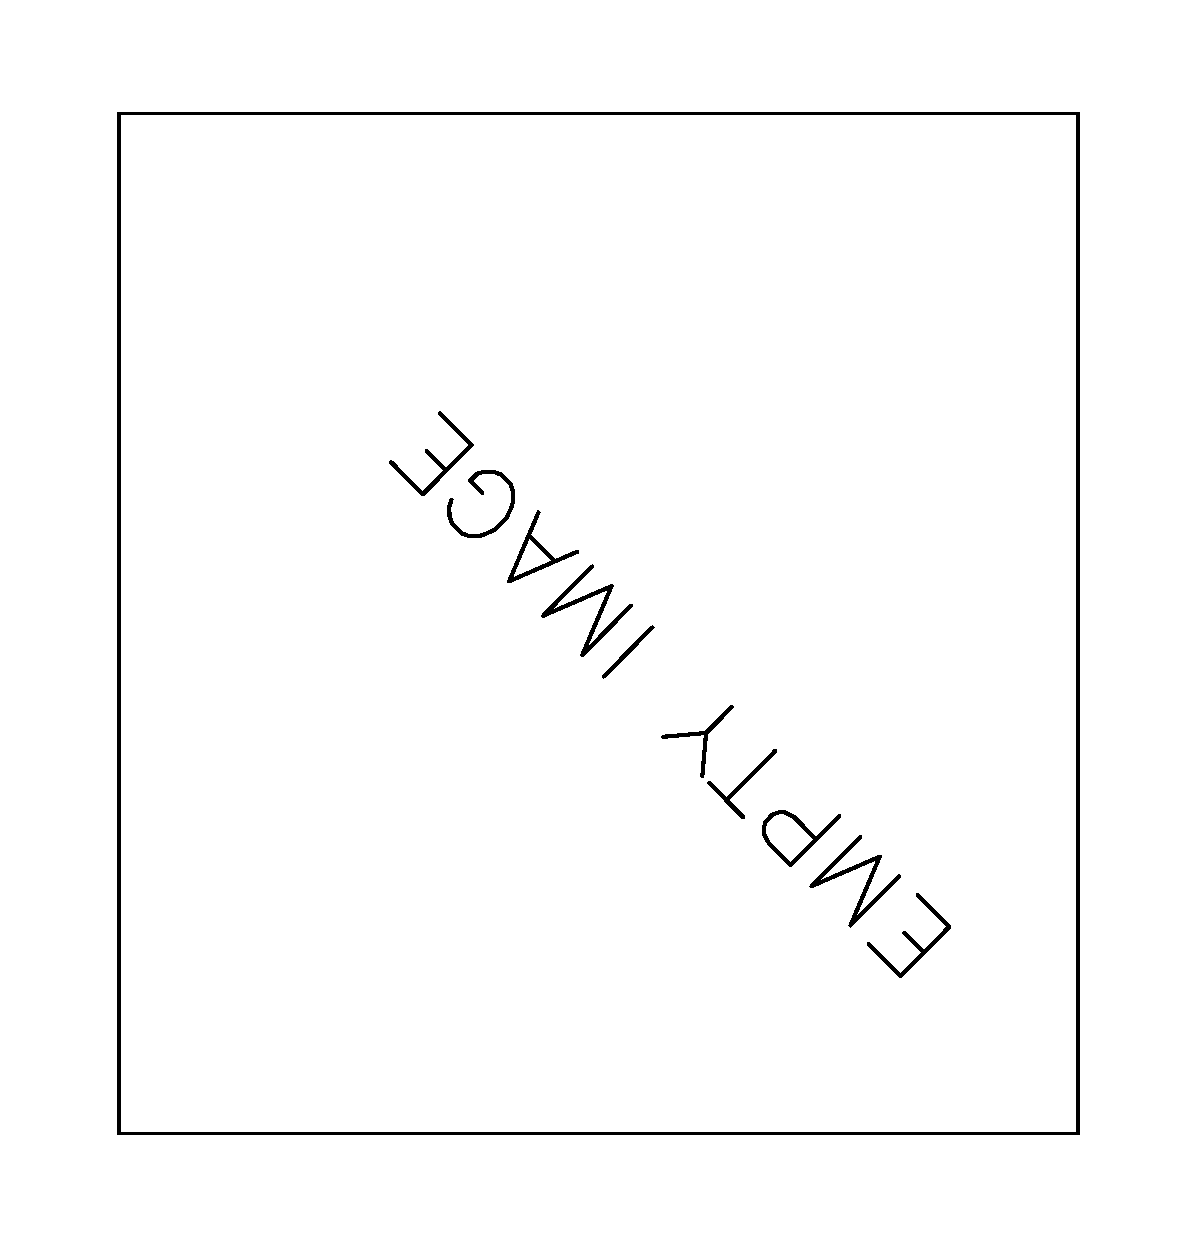
\includegraphics[width=.27\linewidth,angle=-90]{/home/report/FIGS/5GG/1H/emptyimg}}
\subfloat[]{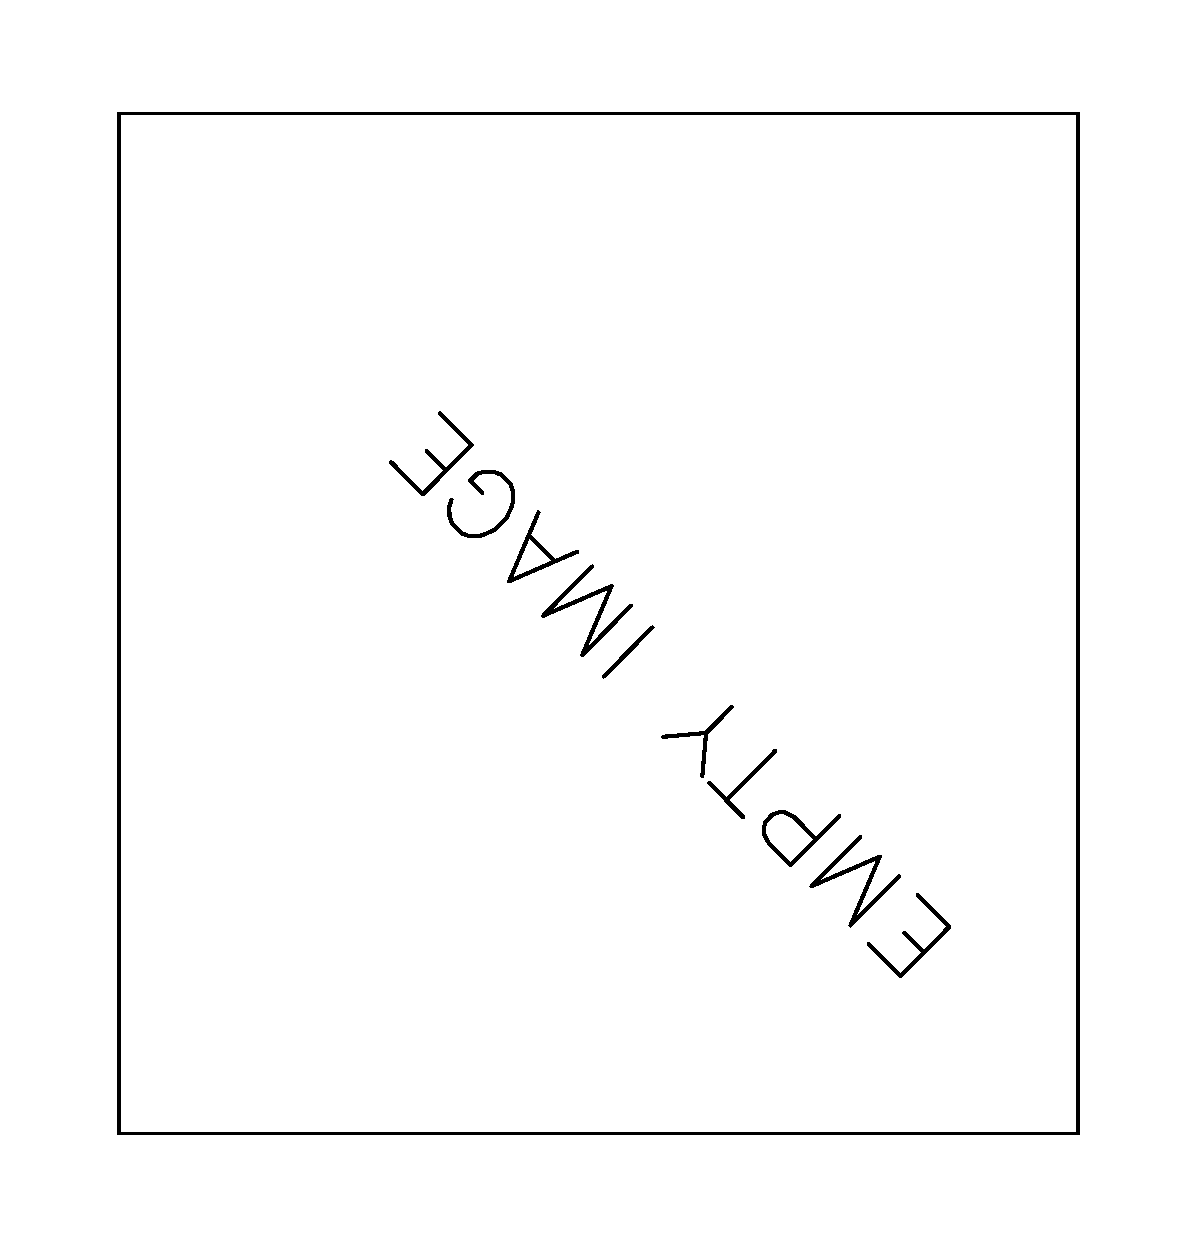
\includegraphics[width=.27\linewidth,angle=-90]{/home/report/FIGS/5GG/1H/emptyimg}}
\caption{TEST-TEST-TEST: (a) STANDARD CONFIGURATION, (b) WITH AR, (c) PERSISTENCE.}
\label{fig:ws}
\end{figure}
%%%%%%%%%%%%%%%%%%%%%%%%%%%%%%%%%
\begin{figure}
\centering
\subfloat[]{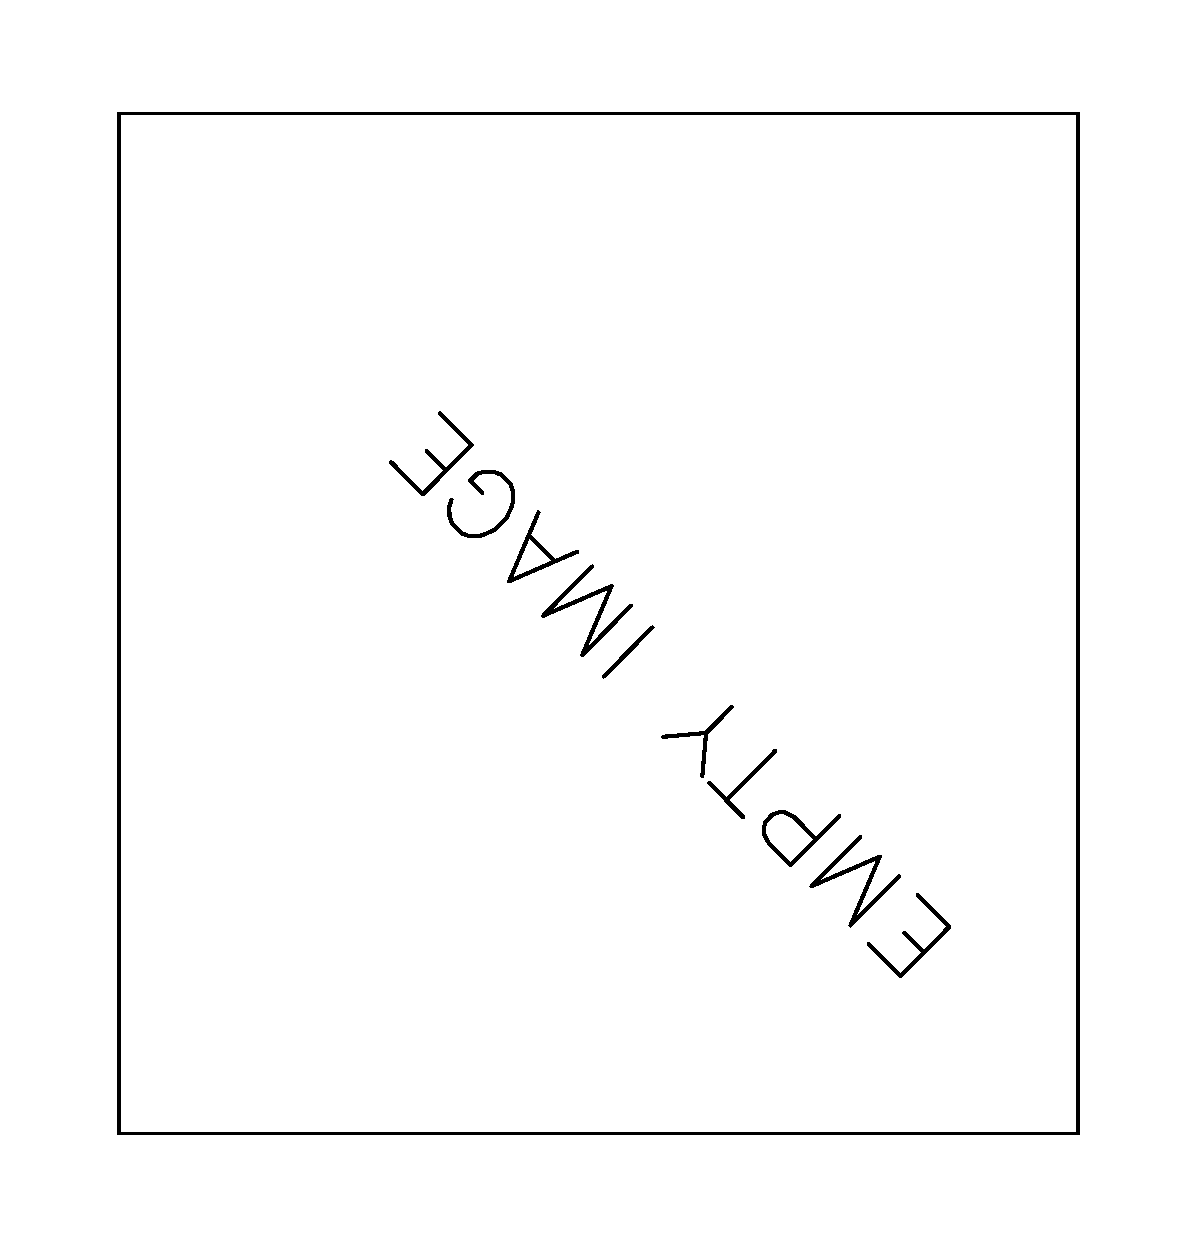
\includegraphics[width=.27\linewidth,angle=-90]{/home/report/FIGS/5GG/1H/emptyimg}}
\subfloat[]{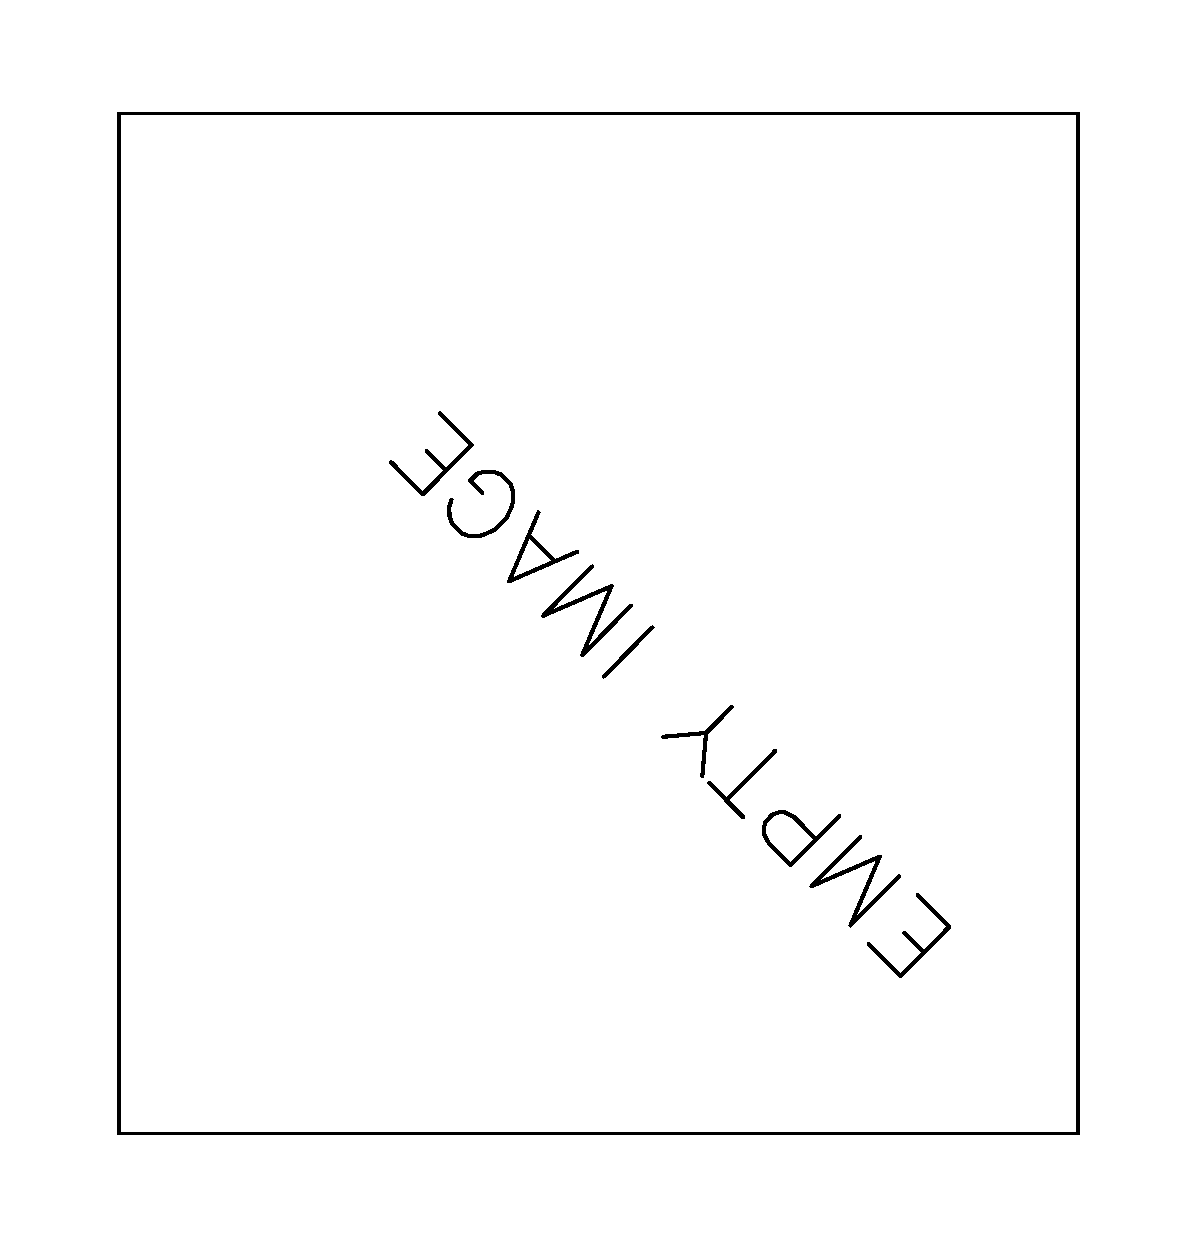
\includegraphics[width=.27\linewidth,angle=-90]{/home/report/FIGS/5GG/1H/emptyimg}}
\subfloat[]{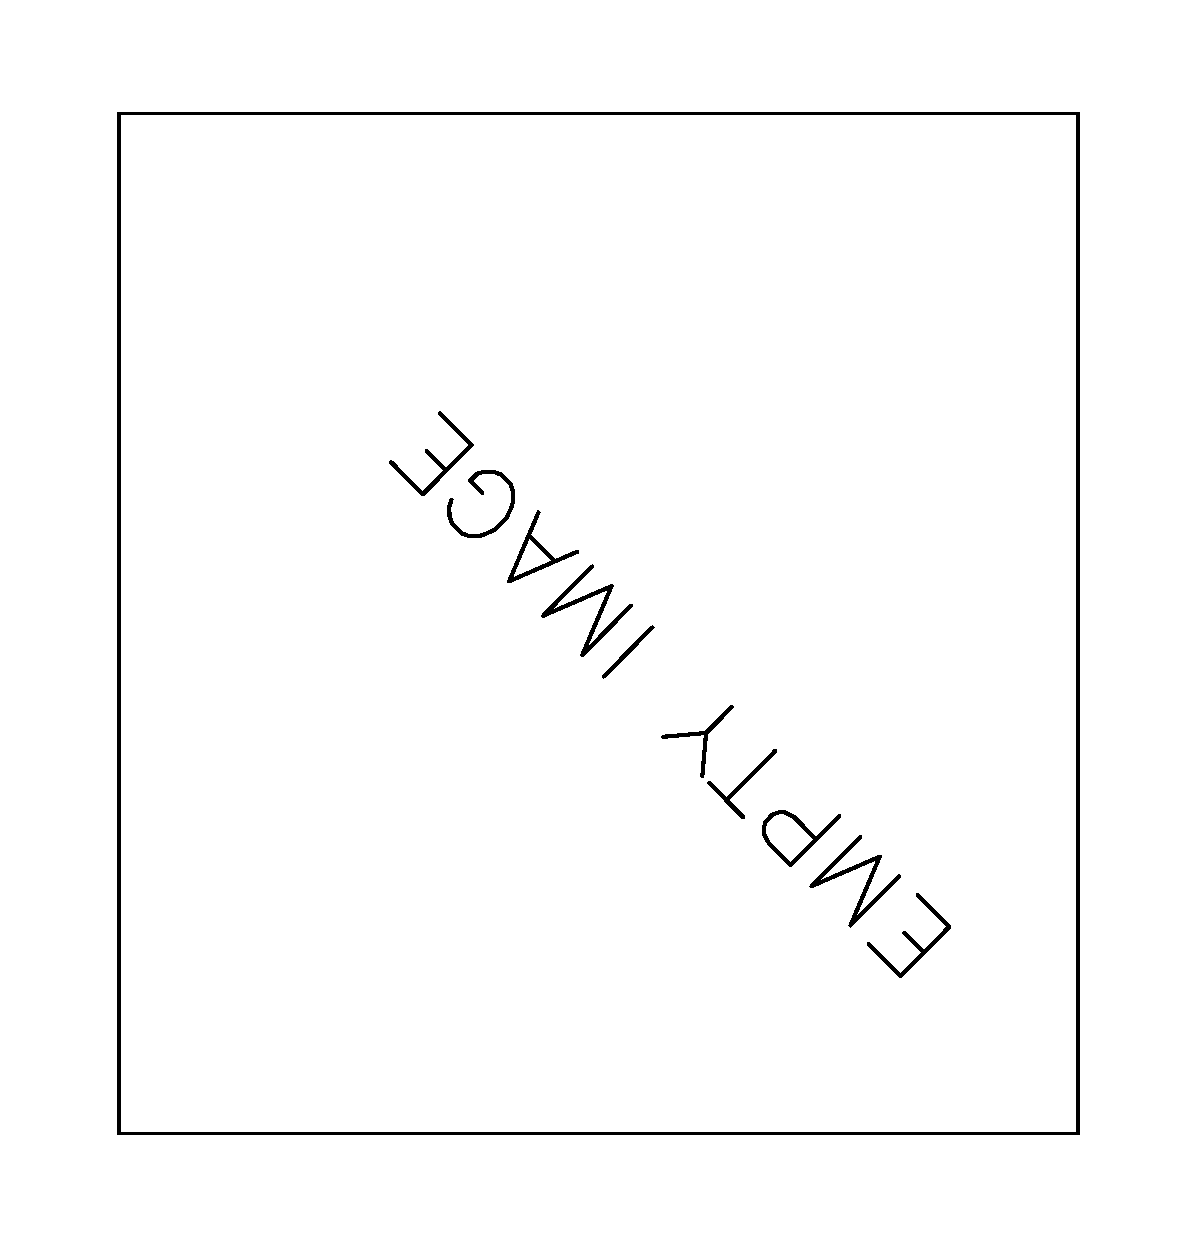
\includegraphics[width=.27\linewidth,angle=-90]{/home/report/FIGS/5GG/1H/emptyimg}}
\caption{TEST-TEST-TEST: (a) STANDARD CONFIGURATION, (b) WITH AR, (c) PERSISTENCE.}
\label{fig:ws}
\end{figure}

%%%%%%%%%%%%%%%%%%%%%%%%%%%%%%%%%
\newpage
%%%%%%%%%%%%%%%%%%%%%%%%%%%%%%%%%

%%%%%%%%%%%%%%%%%%%%
\clearpage
%%%%%%%%%%%%%%%%%%%%
%%%%%%%%%%%%%%%%%%%%%%%%%%%%%%%%%%
%\newpage
\begin{table}[]
\begin{center}
\begin{tabular}{|l|l|l|l|l|l|l|}
\hline
\multicolumn{1}{c|}{\cellcolor[HTML]{C0C0C0}\textbf{VARIABLE}} & \multicolumn{1}{c|}{\cellcolor[HTML]{C0C0C0}\textbf{BIAS} (last month)} & \multicolumn{1}{c|}{\cellcolor[HTML]{C0C0C0}\textbf{RMSE} (last month)} & \multicolumn{1}{c|}{\cellcolor[HTML]{C0C0C0}\textbf{SD} (last month)} & \multicolumn{1}{c|}{\cellcolor[HTML]{C0C0C0}\textbf{BIAS}} & \multicolumn{1}{c|}{\cellcolor[HTML]{C0C0C0}\textbf{RMSE}} & \multicolumn{1}{c|}{\cellcolor[HTML]{C0C0C0}\textbf{SD}}\\\hline
\cellcolor[HTML]{C0C0C0}WS  & WSbiascm     & WSrmsecm     & WSsdcm  &     0.104  &     2.487  &     2.485 \\
\cellcolor[HTML]{C0C0C0}WD  & WDbiascm     & WDrmsecm     & WDsdcm  &   &   &  \\
\cellcolor[HTML]{C0C0C0}RH  & RHbiascm     & RHrmsecm     & RHsdcm  &     0.735  &     6.638  &     6.597 \\
\cellcolor[HTML]{C0C0C0}PWV & PWVbiascm    & PWVrmsecm    & PWVsdcm &    -0.195 &     1.005 &     0.986 \\
\cellcolor[HTML]{C0C0C0}SEE & SEEbiascm    & SEErmsecm    & SEEsdcm &     0.018 &     0.237 &     0.236 \\
\cellcolor[HTML]{C0C0C0}TAU & TAUbiascm    & TAUrmsecm    & TAUsdcm &    -0.073 &     2.221 &     2.220 \\
\cellcolor[HTML]{C0C0C0}GLF & GLFbiascm    & GLFrmsecm    & GLFsdcm &    -0.147 &     0.264 &     0.219 \\
\hline
\end{tabular}
\caption{Statistics for variables in standard configuration}
\end{center}
\end{table}
%%%%%%%%%%%%%%%%%%%%%%%%%%%%%%%%%%
%\newpage
\begin{table}[]
\begin{center}
\begin{tabular}{|l|l|l|l|l|l|l|}
\hline
\multicolumn{1}{c|}{\cellcolor[HTML]{C0C0C0}\textbf{VARIABLE}} & \multicolumn{1}{c|}{\cellcolor[HTML]{C0C0C0}\textbf{BIAS} (last month)} & \multicolumn{1}{c|}{\cellcolor[HTML]{C0C0C0}\textbf{RMSE} (last month)} & \multicolumn{1}{c|}{\cellcolor[HTML]{C0C0C0}\textbf{SD} (last month)} & \multicolumn{1}{c|}{\cellcolor[HTML]{C0C0C0}\textbf{BIAS}} & \multicolumn{1}{c|}{\cellcolor[HTML]{C0C0C0}\textbf{RMSE}} & \multicolumn{1}{c|}{\cellcolor[HTML]{C0C0C0}\textbf{SD}}\\\hline
\cellcolor[HTML]{C0C0C0}WS  & WSbiascm     & WSrmsecm     & WSsdcm  &    -0.010  &     0.659  &     0.659 \\
\cellcolor[HTML]{C0C0C0}WD  & WDbiascm     & WDrmsecm     & WDsdcm  &   &   &  \\
\cellcolor[HTML]{C0C0C0}RH  & RHbiascm     & RHrmsecm     & RHsdcm  &    -0.012  &     1.368  &     1.368 \\
\cellcolor[HTML]{C0C0C0}PWV & PWVbiascm    & PWVrmsecm    & PWVsdcm &    -0.007 &     0.125 &     0.125 \\
\cellcolor[HTML]{C0C0C0}SEE & SEEbiascm    & SEErmsecm    & SEEsdcm &    -0.000 &     0.105 &     0.105 \\
\cellcolor[HTML]{C0C0C0}TAU & TAUbiascm    & TAUrmsecm    & TAUsdcm &    -0.022 &     0.618 &     0.618 \\
\cellcolor[HTML]{C0C0C0}GLF & GLFbiascm    & GLFrmsecm    & GLFsdcm &    -0.007 &     0.067 &     0.067 \\
\hline
\end{tabular}
\caption{Statistics for variables processed with AR (1H)}
\end{center}
\end{table}

%%%%%%%%%%%%%%%%%%%%%%%%%%%%%%%%%
\newpage
%%%%%%%%%%%%%%%%%%%%%%%%%%%%%%%%%

%%%%%%%%%%%%%%%%%%%%
\clearpage
%%%%%%%%%%%%%%%%%%%%
%%%%%%%%%%%%%%%%%%%%%%%%%%%%%%%%%
\begin{table}[]
\begin{center}
\begin{tabular}{llccc}
\hline
{wind speed}                                       &                                                    & \multicolumn{3}{c}{Observations}                 \\
{$m s^{-1}$}                                       &                             & ws $<$ 4.2   & 4.2 $<$ ws $<$ 7.5 & ws $>$ 7.5 \\
\hline
\multicolumn{1}{c}{\multirow{3}{*}{Model data}}  & ws $<$ 4.2             & 4541                & 2127                       & 249              \\
                                                 & 4.2  $<$ ws $<$ 7.5 & 3034                & 3970                       & 1347              \\
                                                 & ws $>$ 7.5             & 430                & 1908                       & 6408              \\
\hline 
\multicolumn{5}{l}{Sample size: 38880; PC=62.1\%; EBD=2.8\%; POD1=56.7\%; POD2=49.6\%; POD3=80.1\%}                 \\
\end{tabular}
\end{center}
\caption{Contingency table for \textbf{wind speed} ($m s^{-1}$) in standard configuration}
\label{tab:contingencywsBEF}
\end{table}
%%%%%%%%%%%%%%%%%%%%%%%%%%%%%%%%%
\begin{table}[]
\begin{center}
\begin{tabular}{llccc}
\hline
{wind speed}                                       &                                                    & \multicolumn{3}{c}{Observations}                 \\
{$m s^{-1}$}                                       &                             & ws $<$ 4.2   & 4.2 $<$ ws $<$ 7.5 & ws $>$ 7.5 \\
\hline
\multicolumn{1}{c}{\multirow{3}{*}{Model data}}  & ws $<$ 4.2             & 7377                & 623                       & 1              \\
                                                 & 4.2  $<$ ws $<$ 7.5 & 628                & 6950                       & 386              \\
                                                 & ws $>$ 7.5             & 0                & 432                       & 7617              \\
\hline 
\multicolumn{5}{l}{Sample size: 38880; PC=91.4\%; EBD=0.0\%; POD1=92.2\%; POD2=86.8\%; POD3=95.2\%}                 \\
\end{tabular}
\end{center}
\caption{Contingency table for variable wind speed ($m s^{-1}$) processed with AR (1H)}
\label{tab:contingencywsAFT}
\end{table}
%%%%%%%%%%%%%%%%%%%%%%%%%%%%%%%%%
\begin{table}[]
\begin{center}
\begin{tabular}{llccc}
\hline
{relative humidity}                                       &                                                    & \multicolumn{3}{c}{Observations}                 \\
{percent}                                       &                             & rh $<$ 7.1   & 7.1 $<$ rh $<$ 15.3 & rh $>$ 15.3 \\
\hline
\multicolumn{1}{c}{\multirow{3}{*}{Model data}}  & rh $<$ 7.1             & 4755                & 1095                       & 27              \\
                                                 & 7.1  $<$ rh $<$ 15.3 & 2696                & 5193                       & 1357              \\
                                                 & rh $>$ 15.3             & 379                & 1539                       & 6443              \\
\hline
\multicolumn{5}{l}{Sample size: 38232; PC=69.8\%; EBD=1.7\%; POD1=60.7\%; POD2=66.3\%; POD3=82.3\%}
\end{tabular}
\end{center}
\caption{Contingency table for variable relative humidity (percent) in standard configuration}
\label{tab:contingencyrhBEF}
\end{table}
%%%%%%%%%%%%%%%%%%%%%%%%%%%%%%%%%
\begin{table}[]
\begin{center}
\begin{tabular}{llccc}
\hline
{relative humidity}                                       &                                                    & \multicolumn{3}{c}{Observations}                 \\
{percent}                                       &                             & rh $<$ 7.1   & 7.1 $<$ rh $<$ 15.3 & rh $>$ 15.3 \\
\hline
\multicolumn{1}{c}{\multirow{3}{*}{Model data}}  & rh $<$ 7.1             & 7408                & 328                       & 1              \\
                                                 & 7.1  $<$ rh $<$ 15.3 & 422                & 7294                       & 248              \\
                                                 & rh $>$ 15.3             & 0                & 205                       & 7578              \\
\hline
\multicolumn{5}{l}{Sample size: 38232; PC=94.9\%; EBD=0.0\%; POD1=94.6\%; POD2=93.2\%; POD3=96.8\%}
\end{tabular}
\end{center}
\caption{Contingency table for variable relative humidity (percent) processed with AR (1H)}
\label{tab:contingencyrhAFT}
\end{table}
%%%%%%%%%%%%%%%%%%%%%%%%%%%%%%%%%
\begin{table}[]
\begin{center}
\begin{tabular}{llccc}
\hline
{precipitable water vapor}                                       &                                                    & \multicolumn{3}{c}{Observations}                 \\
{mm}                                       &                             & pwv $<$ 1.9   & 1.9 $<$ pwv $<$ 3.5 & pwv $>$ 3.5 \\
\hline
\multicolumn{1}{c}{\multirow{3}{*}{Model data}}  & pwv $<$ 1.9             & 3402                & 854                       & 2              \\
                                                 & 1.9  $<$ pwv $<$ 3.5 & 443                & 2596                       & 576              \\
                                                 & pwv $>$ 3.5             & 5                & 400                       & 3271              \\
\hline
\multicolumn{5}{l}{Sample size: 18900; PC=80.3\%; EBD=0.1\%; POD1=88.4\%; POD2=67.4\%; POD3=85.0\%}                 \\
\end{tabular}
\end{center}
\caption{Contingency table for variable precipitable water vapor (mm) in standard configuration}
\label{tab:contingencypwvBEF}
\end{table}
%%%%%%%%%%%%%%%%%%%%%%%%%%%%%%%%%
\begin{table}[]
\begin{center}
\begin{tabular}{llccc}
\hline
{precipitable water vapor}                                       &                                                    & \multicolumn{3}{c}{Observations}                 \\
{mm}                                       &                             & pwv $<$ 1.9   & 1.9 $<$ pwv $<$ 3.5 & pwv $>$ 3.5 \\
\hline
\multicolumn{1}{c}{\multirow{3}{*}{Model data}}  & pwv $<$ 1.9             & 3785                & 69                       & 0              \\
                                                 & 1.9  $<$ pwv $<$ 3.5 & 65                & 3733                       & 39              \\
                                                 & pwv $>$ 3.5             & 0                & 48                       & 3810              \\
\hline 
\multicolumn{5}{l}{Sample size: 18900; PC=98.1\%; EBD=0.0\%; POD1=98.3\%; POD2=97.0\%; POD3=99.0\%}
\end{tabular}
\end{center}
\caption{Contingency table for variable precipitable water vapor (mm) processed with AR (1H)}
\label{tab:contingencypwvAFT}
\end{table}
%%%%%%%%%%%%%%%%%%%%
\clearpage
%%%%%%%%%%%%%%%%%%%%
%%%%%%%%%%%%%%%%%%%%%%%%%%%%%%%%%
\begin{table}[]
\begin{center}
\begin{tabular}{llccc}
\hline
{total seeing}                                       &                                                    & \multicolumn{3}{c}{Observations}                 \\
{arcsec}                                       &                             & see $<$ 0.6
0.6   & 0.6
0.6 $<$ see $<$ 0.8
0.8 & see $>$ 0.8
0.8 \\
\hline
\multicolumn{1}{c}{\multirow{3}{*}{Model data}}  & see $<$ 0.6
0.6             & 2465                & 1647                       & 534              \\
                                                 & 0.6
0.6  $<$ see $<$ 0.8
0.8 & 2812                & 2819                       & 1947              \\
                                                 & see $>$ 0.8
0.8             & 749                & 1559                       & 3544              \\
\hline
\multicolumn{5}{l}{Sample size: 37584; PC=48.8\%; EBD=7.1\%; POD1=40.9\%; POD2=46.8\%; POD3=58.8\%}
\end{tabular}
\end{center}
\caption{Contingency table for variable total seeing (arcsec) in standard configuration and accuracy 0.0}
\label{tab:contingencyseeBEF}
\end{table}
%%%%%%%%%%%%%%%%%%%%%%%%%%%%%%%%%
\begin{table}[]
\begin{center}
\begin{tabular}{llccc}
\hline
{total seeing}                                       &                                                    & \multicolumn{3}{c}{Observations}                 \\
{arcsec}                                       &                             & see $<$ 0.6
0.6   & 0.6
0.6 $<$ see $<$ 0.8
0.8 & see $>$ 0.8
0.8 \\
\hline
\multicolumn{1}{c}{\multirow{3}{*}{Model data}}  & see $<$ 0.6
0.6             & 4356                & 308                       & 1423              \\
                                                 & 0.6
0.6  $<$ see $<$ 0.8
0.8 & 921                & 4766                       & 1411              \\
                                                 & see $>$ 0.8
0.8             & 749                & 951                       & 4527              \\
\hline
\multicolumn{5}{l}{Sample size: 37584; PC=75.5\%; EBD=12.0\%; POD1=72.3\%; POD2=79.1\%; POD3=61.5\%}
\end{tabular}
\end{center}
\caption{Contingency table for variable total seeing (arcsec) in standard configuration and accuracy 0.10}
\label{tab:contingencyseeBEF}
\end{table}
%%%%%%%%%%%%%%%%%%%%%%%%%%%%%%%%%
\begin{table}[]
\begin{center}
\begin{tabular}{llccc}
\hline
{total seeing}                                       &                                                    & \multicolumn{3}{c}{Observations}                 \\
{arcsec}                                       &                             & see $<$ 0.6
0.6   & 0.6
0.6 $<$ see $<$ 0.8
0.8 & see $>$ 0.8
0.8 \\
\hline
\multicolumn{1}{c}{\multirow{3}{*}{Model data}}  & see $<$ 0.6
0.6             & 5456                & 0                       & 329              \\
                                                 & 0.6
0.6  $<$ see $<$ 0.8
0.8 & 0                & 5613                       & 329              \\
                                                 & see $>$ 0.8
0.8             & 570                & 412                       & 5696              \\
\hline
\multicolumn{5}{l}{Sample size: 37584; PC=92.7\%; EBD=5.0\%; POD1=90.5\%; POD2=93.2\%; POD3=89.6\%}
\end{tabular}
\end{center}
\caption{Contingency table for variable total seeing (arcsec) in standard configuration and accuracy 0.24}
\label{tab:contingencyseeBEF}
\end{table}
%%%%%%%%%%%%%%%%%%%%%%%%%%%%%%%%%
\begin{table}[]
\begin{center}
\begin{tabular}{llccc}
\hline
{total seeing}                                       &                                                    & \multicolumn{3}{c}{Observations}                 \\
{arcsec}                                       &                             & see $<$ 0.6
0.6   & 0.6
0.6 $<$ see $<$ 0.8
0.8 & see $>$ 0.8
0.8 \\
\hline
\multicolumn{1}{c}{\multirow{3}{*}{Model data}}  & see $<$ 0.6
0.6             & 5670                & 816                       & 27              \\
                                                 & 0.6
0.6  $<$ see $<$ 0.8
0.8 & 765                & 4910                       & 535              \\
                                                 & see $>$ 0.8
0.8             & 11                & 720                       & 5884              \\
\hline
\multicolumn{5}{l}{Sample size: 37584; PC=85.1\%; EBD=0.2\%; POD1=88.0\%; POD2=76.2\%; POD3=91.3\%}
\end{tabular}
\end{center}
\caption{Contingency table for variable total seeing (arcsec) processed with AR (1H) and accuracy 0.0}
\label{tab:contingencyseeAFT}
\end{table}
%%%%%%%%%%%%%%%%%%%%%%%%%%%%%%%%%
\begin{table}[]
\begin{center}
\begin{tabular}{llccc}
\hline
{total seeing}                                       &                                                    & \multicolumn{3}{c}{Observations}                 \\
{arcsec}                                       &                             & see $<$ 0.6
0.6   & 0.6
0.6 $<$ see $<$ 0.8
0.8 & see $>$ 0.8
0.8 \\
\hline
\multicolumn{1}{c}{\multirow{3}{*}{Model data}}  & see $<$ 0.6
0.6             & 6321                & 156                       & 91              \\
                                                 & 0.6
0.6  $<$ see $<$ 0.8
0.8 & 114                & 6117                       & 118              \\
                                                 & see $>$ 0.8
0.8             & 11                & 173                       & 6317              \\
\hline
\multicolumn{5}{l}{Sample size: 37584; PC=97.0\%; EBD=0.5\%; POD1=98.1\%; POD2=94.9\%; POD3=96.8\%}
\end{tabular}
\end{center}
\caption{Contingency table for variable total seeing (arcsec) processed with AR (1H) and accuracy 0.10}
\label{tab:contingencyseeAFT}
\end{table}
%%%%%%%%%%%%%%%%%%%%%%%%%%%%%%%%%
\begin{table}[]
\begin{center}
\begin{tabular}{llccc}
\hline
{total seeing}                                       &                                                    & \multicolumn{3}{c}{Observations}                 \\
{arcsec}                                       &                             & see $<$ 0.6
0.6   & 0.6
0.6 $<$ see $<$ 0.8
0.8 & see $>$ 0.8
0.8 \\
\hline
\multicolumn{1}{c}{\multirow{3}{*}{Model data}}  & see $<$ 0.6
0.6             & 6436                & 13                       & 24              \\
                                                 & 0.6
0.6  $<$ see $<$ 0.8
0.8 & 0                & 6401                       & 18              \\
                                                 & see $>$ 0.8
0.8             & 10                & 32                       & 6422              \\
\hline
\multicolumn{5}{l}{Sample size: 37584; PC=99.6\%; EBD=0.2\%; POD1=99.8\%; POD2=99.3\%; POD3=99.4\%}
\end{tabular}
\end{center}
\caption{Contingency table for variable total seeing (arcsec) processed with AR (1H) and accuracy 0.24}
\label{tab:contingencyseeAFT}
\end{table}
%%%%%%%%%%%%%%%%%%%%%%%%%%%%%%%%%
\begin{table}[]
\begin{center}
\begin{tabular}{llccc}
\hline
{coeherence time}                                       &                                                    & \multicolumn{3}{c}{Observations}                 \\
{ms}                                       &                             & tau $<$ 3.4   & 3.4 $<$ tau $<$ 5.8 & tau $>$ 5.8 \\
\hline
\multicolumn{1}{c}{\multirow{3}{*}{Model data}}  & tau $<$ 3.4             & 3678                & 872                       & 99              \\
                                                 & 3.4  $<$ tau $<$ 5.8 & 1794                & 3570                       & 2015              \\
                                                 & tau $>$ 5.8             & 281                & 1311                       & 3639              \\
\hline
\multicolumn{5}{l}{Sample size: 37476; PC=63.1\%; EBD=2.2\%; POD1=63.9\%; POD2=62.1\%; POD3=63.3\%}
\end{tabular}
\end{center}
\caption{Contingency table for variable coeherence time (ms) in standard configuration and accuracy 0.0}
\label{tab:contingencytauBEF}
\end{table}
%%%%%%%%%%%%%%%%%%%%%%%%%%%%%%%%%
\begin{table}[]
\begin{center}
\begin{tabular}{llccc}
\hline
{coeherence time}                                       &                                                    & \multicolumn{3}{c}{Observations}                 \\
{ms}                                       &                             & tau $<$ 3.4   & 3.4 $<$ tau $<$ 5.8 & tau $>$ 5.8 \\
\hline
\multicolumn{1}{c}{\multirow{3}{*}{Model data}}  & tau $<$ 3.4             & 5012                & 61                       & 747              \\
                                                 & 3.4  $<$ tau $<$ 5.8 & 460                & 5126                       & 747              \\
                                                 & tau $>$ 5.8             & 281                & 566                       & 5006              \\
\hline
\multicolumn{5}{l}{Sample size: 37476; PC=87.7\%; EBD=6.0\%; POD1=87.1\%; POD2=89.1\%; POD3=77.0\%}
\end{tabular}
\end{center}
\caption{Contingency table for variable coeherence time (ms) in standard configuration and accuracy 1.22}
\label{tab:contingencytauBEF}
\end{table}
%%%%%%%%%%%%%%%%%%%%%%%%%%%%%%%%%
\begin{table}[]
\begin{center}
\begin{tabular}{llccc}
\hline
{coeherence time}                                       &                                                    & \multicolumn{3}{c}{Observations}                 \\
{ms}                                       &                             & tau $<$ 3.4   & 3.4 $<$ tau $<$ 5.8 & tau $>$ 5.8 \\
\hline
\multicolumn{1}{c}{\multirow{3}{*}{Model data}}  & tau $<$ 3.4             & 5349                & 369                       & 1              \\
                                                 & 3.4  $<$ tau $<$ 5.8 & 401                & 4970                       & 417              \\
                                                 & tau $>$ 5.8             & 3                & 414                       & 5335              \\
\hline
\multicolumn{5}{l}{Sample size: 37476; PC=90.7\%; EBD=0.0\%; POD1=93.0\%; POD2=86.4\%; POD3=92.7\%}
\end{tabular}
\end{center}
\caption{Contingency table for variable coeherence time (ms) processed with AR (1H) and accuracy 0.0}
\label{tab:contingencytauAFT}
\end{table}
%%%%%%%%%%%%%%%%%%%%%%%%%%%%%%%%%
\begin{table}[]
\begin{center}
\begin{tabular}{llccc}
\hline
{coeherence time}                                       &                                                    & \multicolumn{3}{c}{Observations}                 \\
{ms}                                       &                             & tau $<$ 3.4   & 3.4 $<$ tau $<$ 5.8 & tau $>$ 5.8 \\
\hline
\multicolumn{1}{c}{\multirow{3}{*}{Model data}}  & tau $<$ 3.4             & 5742                & 2                       & 28              \\
                                                 & 3.4  $<$ tau $<$ 5.8 & 8                & 5714                       & 28              \\
                                                 & tau $>$ 5.8             & 3                & 37                       & 5725              \\
\hline
\multicolumn{5}{l}{Sample size: 37476; PC=99.5\%; EBD=0.2\%; POD1=99.8\%; POD2=99.3\%; POD3=99.0\%}
\end{tabular}
\end{center}
\caption{Contingency table for variable coeherence time (ms) processed with AR (1H) and accuracy 1.22}
\label{tab:contingencytauAFT}
\end{table}
%%%%%%%%%%%%%%%%%%%%%%%%%%%%%%%%%
\begin{table}[]
\begin{center}
\begin{tabular}{llccc}
\hline
{ground layer fraction}                                       &                                                    & \multicolumn{3}{c}{Observations}                 \\
{dimensionless}                                       &                             & glf $<$ 0.6   & 0.6 $<$ glf $<$ 0.7 & glf $>$ 0.7 \\
\hline
\multicolumn{1}{c}{\multirow{3}{*}{Model data}}  & glf $<$ 0.6             & 4369                & 3882                       & 3308              \\
                                                 & 0.6  $<$ glf $<$ 0.7 & 1034                & 1283                       & 1478              \\
                                                 & glf $>$ 0.7             & 354                & 592                       & 970              \\
\hline
\multicolumn{5}{l}{Sample size: 37476; PC=38.3\%; EBD=21.2\%; POD1=75.9\%; POD2=22.3\%; POD3=16.9\%}
\end{tabular}
\end{center}
\caption{Contingency table for variable ground layer fraction (dimensionless) in standard configuration and accuracy 0.0}
\label{tab:contingencyglfBEF}
\end{table}
%%%%%%%%%%%%%%%%%%%%%%%%%%%%%%%%%
\begin{table}[]
\begin{center}
\begin{tabular}{llccc}
\hline
{ground layer fraction}                                       &                                                    & \multicolumn{3}{c}{Observations}                 \\
{dimensionless}                                       &                             & glf $<$ 0.6   & 0.6 $<$ glf $<$ 0.7 & glf $>$ 0.7 \\
\hline
\multicolumn{1}{c}{\multirow{3}{*}{Model data}}  & glf $<$ 0.6             & 5353                & 2517                       & 3403              \\
                                                 & 0.6  $<$ glf $<$ 0.7 & 50                & 3223                       & 1436              \\
                                                 & glf $>$ 0.7             & 354                & 17                       & 2353              \\
\hline
\multicolumn{5}{l}{Sample size: 37476; PC=63.3\%; EBD=21.8\%; POD1=93.0\%; POD2=56.0\%; POD3=32.7\%}
\end{tabular}
\end{center}
\caption{Contingency table for variable ground layer fraction (dimensionless) in standard configuration and accuracy 0.14}
\label{tab:contingencyglfBEF}
\end{table}
%%%%%%%%%%%%%%%%%%%%%%%%%%%%%%%%%
\begin{table}[]
\begin{center}
\begin{tabular}{llccc}
\hline
{ground layer fraction}                                       &                                                    & \multicolumn{3}{c}{Observations}                 \\
{dimensionless}                                       &                             & glf $<$ 0.6   & 0.6 $<$ glf $<$ 0.7 & glf $>$ 0.7 \\
\hline
\multicolumn{1}{c}{\multirow{3}{*}{Model data}}  & glf $<$ 0.6             & 5041                & 935                       & 43              \\
                                                 & 0.6  $<$ glf $<$ 0.7 & 676                & 4140                       & 904              \\
                                                 & glf $>$ 0.7             & 40                & 682                       & 4809              \\
\hline
\multicolumn{5}{l}{Sample size: 37476; PC=81.0\%; EBD=0.5\%; POD1=87.6\%; POD2=71.9\%; POD3=83.5\%}
\end{tabular}
\end{center}
\caption{Contingency table for variable ground layer fraction (dimensionless) processed with AR (1H) and accuracy 0.0}
\label{tab:contingencyglfAFT}
\end{table}
%%%%%%%%%%%%%%%%%%%%%%%%%%%%%%%%%
\begin{table}[]
\begin{center}
\begin{tabular}{llccc}
\hline
{ground layer fraction}                                       &                                                    & \multicolumn{3}{c}{Observations}                 \\
{dimensionless}                                       &                             & glf $<$ 0.6   & 0.6 $<$ glf $<$ 0.7 & glf $>$ 0.7 \\
\hline
\multicolumn{1}{c}{\multirow{3}{*}{Model data}}  & glf $<$ 0.6             & 5712                & 74                       & 55              \\
                                                 & 0.6  $<$ glf $<$ 0.7 & 5                & 5658                       & 54              \\
                                                 & glf $>$ 0.7             & 40                & 25                       & 5701              \\
\hline
\multicolumn{5}{l}{Sample size: 37476; PC=98.8\%; EBD=0.6\%; POD1=99.2\%; POD2=98.3\%; POD3=98.1\%}
\end{tabular}
\end{center}
\caption{Contingency table for variable ground layer fraction (dimensionless) processed with AR (1H) and accuracy 0.14}
\label{tab:contingencyglfAFT}
\end{table}
%%%%%%%%%%%%%%%%%%%%
\clearpage
%%%%%%%%%%%%%%%%%%%%

%%%%%%%%%%%%%%%%%%%%%%%%%%%%%%%%%
\newpage
%%%%%%%%%%%%%%%%%%%%%%%%%%%%%%%%%

%%%%%%%%%%%%%%%%%%%%
\clearpage
%%%%%%%%%%%%%%%%%%%%
%%%%%%%%%%%%%%%%%%%%%%%%%%%%%%%%%%
\begin{table}[]
\begin{center}
\begin{tabular}{|l|l|l|l|}
\hline
\multicolumn{1}{|c|}{\cellcolor[HTML]{C0C0C0}\textbf{PARAMETER}} & \multicolumn{1}{c|}{\cellcolor[HTML]{C0C0C0}\textbf{STANDARD}} & \multicolumn{1}{c|}{\cellcolor[HTML]{C0C0C0}\textbf{WITH AR (1H)}} \\
\hline
\cellcolor[HTML]{C0C0C0}POD1  & 56.7                                & 92.2         \\
\cellcolor[HTML]{C0C0C0}POD2  & 49.6                                & 86.8         \\
\cellcolor[HTML]{C0C0C0}POD3  & 80.1                                & 95.2         \\
\cellcolor[HTML]{C0C0C0}PC    & 62.1                                  & 91.4           \\
\cellcolor[HTML]{C0C0C0}EBD   & 2.8                                 & 0.0          \\
\hline
\end{tabular}
\caption{PODs for wind speed ($m s^{-1}$)}
\end{center}
\end{table}
%%%%%%%%%%%%%%%%%%%%%%%%%%%%%%%%%%
\begin{table}[]
\begin{center}
\begin{tabular}{|l|l|l|l|}
\hline
\multicolumn{1}{|c|}{\cellcolor[HTML]{C0C0C0}\textbf{PARAMETER}} & \multicolumn{1}{c|}{\cellcolor[HTML]{C0C0C0}\textbf{STANDARD}} & \multicolumn{1}{c|}{\cellcolor[HTML]{C0C0C0}\textbf{WITH AR (1H)}} \\
\hline
\cellcolor[HTML]{C0C0C0}POD1  & 60.7                                & 94.6         \\
\cellcolor[HTML]{C0C0C0}POD2  & 66.3                                & 93.2         \\
\cellcolor[HTML]{C0C0C0}POD3  & 82.3                                & 96.8         \\
\cellcolor[HTML]{C0C0C0}PC    & 69.8                                  & 94.9           \\
\cellcolor[HTML]{C0C0C0}EBD   & 1.7                                 & 0.0          \\
\hline
\end{tabular}
\caption{PODs for relative humidity (percent)}
\end{center}
\end{table}
%%%%%%%%%%%%%%%%%%%%%%%%%%%%%%%%%%
\begin{table}[]
\begin{center}
\begin{tabular}{|l|l|l|l|}
\hline
\multicolumn{1}{|c|}{\cellcolor[HTML]{C0C0C0}\textbf{PARAMETER}} & \multicolumn{1}{c|}{\cellcolor[HTML]{C0C0C0}\textbf{STANDARD}} & \multicolumn{1}{c|}{\cellcolor[HTML]{C0C0C0}\textbf{WITH AR (1H)}} \\
\hline
\cellcolor[HTML]{C0C0C0}POD1  & 88.4                                & 98.3         \\
\cellcolor[HTML]{C0C0C0}POD2  & 67.4                                & 97.0         \\
\cellcolor[HTML]{C0C0C0}POD3  & 85.0                                & 99.0         \\
\cellcolor[HTML]{C0C0C0}PC    & 80.3                                  & 98.1           \\
\cellcolor[HTML]{C0C0C0}EBD   & 0.1                                 & 0.0          \\
\hline
\end{tabular}
\caption{PODs for precipitable water vapor (mm)}
\end{center}
\end{table}
%%%%%%%%%%%%%%%%%%%%%%%%%%%%%%%%%%
\begin{table}[]
\begin{center}
\begin{tabular}{|l|l|l|l|}
\hline
\multicolumn{1}{|c|}{\cellcolor[HTML]{C0C0C0}\textbf{PARAMETER}} & \multicolumn{1}{c|}{\cellcolor[HTML]{C0C0C0}\textbf{STANDARD}} & \multicolumn{1}{c|}{\cellcolor[HTML]{C0C0C0}\textbf{WITH AR (1H)}} \\
\hline
\cellcolor[HTML]{C0C0C0}POD1  & 40.9                                & 88.0         \\
\cellcolor[HTML]{C0C0C0}POD2  & 46.8                                & 76.2         \\
\cellcolor[HTML]{C0C0C0}POD3  & 58.8                                & 91.3         \\
\cellcolor[HTML]{C0C0C0}PC    & 48.8                                  & 85.1           \\
\cellcolor[HTML]{C0C0C0}EBD   & 7.1                                 & 0.2          \\
\hline
\end{tabular}
\caption{PODs for total seeing (arcsec) and accuray 0.0}
\end{center}
\end{table}
%%%%%%%%%%%%%%%%%%%%%%%%%%%%%%%%%%
\begin{table}[]
\begin{center}
\begin{tabular}{|l|l|l|l|}
\hline
\multicolumn{1}{|c|}{\cellcolor[HTML]{C0C0C0}\textbf{PARAMETER}} & \multicolumn{1}{c|}{\cellcolor[HTML]{C0C0C0}\textbf{STANDARD}} & \multicolumn{1}{c|}{\cellcolor[HTML]{C0C0C0}\textbf{WITH AR (1H)}} \\
\hline
\cellcolor[HTML]{C0C0C0}POD1  & 72.3                                & 98.1         \\
\cellcolor[HTML]{C0C0C0}POD2  & 79.1                                & 94.9         \\
\cellcolor[HTML]{C0C0C0}POD3  & 61.5                                & 96.8         \\
\cellcolor[HTML]{C0C0C0}PC    & 75.5                                  & 97.0           \\
\cellcolor[HTML]{C0C0C0}EBD   & 12.0                                 & 0.5          \\
\hline
\end{tabular}
\caption{PODs for total seeing (arcsec) and accuray 0.10}
\end{center}
\end{table}
%%%%%%%%%%%%%%%%%%%%%%%%%%%%%%%%%%
\begin{table}[]
\begin{center}
\begin{tabular}{|l|l|l|l|}
\hline
\multicolumn{1}{|c|}{\cellcolor[HTML]{C0C0C0}\textbf{PARAMETER}} & \multicolumn{1}{c|}{\cellcolor[HTML]{C0C0C0}\textbf{STANDARD}} & \multicolumn{1}{c|}{\cellcolor[HTML]{C0C0C0}\textbf{WITH AR (1H)}} \\
\hline
\cellcolor[HTML]{C0C0C0}POD1  & 90.5                                & 99.8         \\
\cellcolor[HTML]{C0C0C0}POD2  & 93.2                                & 99.3         \\
\cellcolor[HTML]{C0C0C0}POD3  & 89.6                                & 99.4         \\
\cellcolor[HTML]{C0C0C0}PC    & 92.7                                  & 99.6           \\
\cellcolor[HTML]{C0C0C0}EBD   & 5.0                                 & 0.2          \\
\hline
\end{tabular}
\caption{PODs for total seeing (arcsec) and accuray 0.24}
\end{center}
\end{table}
%%%%%%%%%%%%%%%%%%%%%%%%%%%%%%%%%%
\begin{table}[]
\begin{center}
\begin{tabular}{|l|l|l|l|}
\hline
\multicolumn{1}{|c|}{\cellcolor[HTML]{C0C0C0}\textbf{PARAMETER}} & \multicolumn{1}{c|}{\cellcolor[HTML]{C0C0C0}\textbf{STANDARD}} & \multicolumn{1}{c|}{\cellcolor[HTML]{C0C0C0}\textbf{WITH AR (1H)}} \\
\hline
\cellcolor[HTML]{C0C0C0}POD1  & 63.9                                & 93.0         \\
\cellcolor[HTML]{C0C0C0}POD2  & 62.1                                & 86.4         \\
\cellcolor[HTML]{C0C0C0}POD3  & 63.3                                & 92.7         \\
\cellcolor[HTML]{C0C0C0}PC    & 63.1                                  & 90.7           \\
\cellcolor[HTML]{C0C0C0}EBD   & 2.2                                 & 0.0          \\
\hline
\end{tabular}
\caption{PODs for coeherence time (ms) and accuray 0.0}
\end{center}
\end{table}
%%%%%%%%%%%%%%%%%%%%%%%%%%%%%%%%%%
\begin{table}[]
\begin{center}
\begin{tabular}{|l|l|l|l|}
\hline
\multicolumn{1}{|c|}{\cellcolor[HTML]{C0C0C0}\textbf{PARAMETER}} & \multicolumn{1}{c|}{\cellcolor[HTML]{C0C0C0}\textbf{STANDARD}} & \multicolumn{1}{c|}{\cellcolor[HTML]{C0C0C0}\textbf{WITH AR (1H)}} \\
\hline
\cellcolor[HTML]{C0C0C0}POD1  & 87.1                                & 99.8         \\
\cellcolor[HTML]{C0C0C0}POD2  & 89.1                                & 99.3         \\
\cellcolor[HTML]{C0C0C0}POD3  & 77.0                                & 99.0         \\
\cellcolor[HTML]{C0C0C0}PC    & 87.7                                  & 99.5           \\
\cellcolor[HTML]{C0C0C0}EBD   & 6.0                                 & 0.2          \\
\hline
\end{tabular}
\caption{PODs for coeherence time (ms) and accuray 1.22}
\end{center}
\end{table}
%%%%%%%%%%%%%%%%%%%%%%%%%%%%%%%%%%
\begin{table}[]
\begin{center}
\begin{tabular}{|l|l|l|l|}
\hline
\multicolumn{1}{|c|}{\cellcolor[HTML]{C0C0C0}\textbf{PARAMETER}} & \multicolumn{1}{c|}{\cellcolor[HTML]{C0C0C0}\textbf{STANDARD}} & \multicolumn{1}{c|}{\cellcolor[HTML]{C0C0C0}\textbf{WITH AR (1H)}} \\
\hline
\cellcolor[HTML]{C0C0C0}POD1  & 75.9                                & 87.6         \\
\cellcolor[HTML]{C0C0C0}POD2  & 22.3                                & 71.9         \\
\cellcolor[HTML]{C0C0C0}POD3  & 16.9                                & 83.5         \\
\cellcolor[HTML]{C0C0C0}PC    & 38.3                                  & 81.0           \\
\cellcolor[HTML]{C0C0C0}EBD   & 21.2                                 & 0.5          \\
\hline
\end{tabular}
\caption{PODs for ground layer fraction (dimensionless) and accuray 0.0}
\end{center}
\end{table}
%%%%%%%%%%%%%%%%%%%%%%%%%%%%%%%%%%
\begin{table}[]
\begin{center}
\begin{tabular}{|l|l|l|l|}
\hline
\multicolumn{1}{|c|}{\cellcolor[HTML]{C0C0C0}\textbf{PARAMETER}} & \multicolumn{1}{c|}{\cellcolor[HTML]{C0C0C0}\textbf{STANDARD}} & \multicolumn{1}{c|}{\cellcolor[HTML]{C0C0C0}\textbf{WITH AR (1H)}} \\
\hline
\cellcolor[HTML]{C0C0C0}POD1  & 93.0                                & 99.2         \\
\cellcolor[HTML]{C0C0C0}POD2  & 56.0                                & 98.3         \\
\cellcolor[HTML]{C0C0C0}POD3  & 32.7                                & 98.1         \\
\cellcolor[HTML]{C0C0C0}PC    & 63.3                                  & 98.8           \\
\cellcolor[HTML]{C0C0C0}EBD   & 21.8                                 & 0.6          \\
\hline
\end{tabular}
\caption{PODs for ground layer fraction (dimensionless) and accuray 0.14}
\end{center}
\end{table}

%%%%%%%%%%%%%%%%%%%%%%%%%%%%%%%%%
\clearpage
%\begin{center}
%\HRule \\[0.4cm]
%\begin{figure}[htbp]
%\centering
%{
\includegraphics[width=2.5cm]{/home/report/scripts/LOGOS/fate_logo_11def}}
%\caption{Add some meaningfull logo or figure here}
%\end{figure}
%\HRule \\[0.4cm]
%\end{center}

%\section{Contacts}
\vspace{1.5cm}
\begin{flushleft}
\HRule \\[0.4cm]
{
\includegraphics[width=2.5cm]{/home/report/SCRIPTS/LOGOS/fate_logo_11def}}
\\
\Large{For any further information or questions please contact:
\\ WHO
\\ ADDRESS1
\\ ADDRESS2
\\ EMAIL: \href{mailto:e.musk@lamma.toscana.it}{e.musk@lamma.toscana.it}
\\ WEB: \href{www.lamma.toscana.com}{www.lamma.toscana.com}
\\ PHONE: MY\_PHONE
\\ FAX: MY\_FAX(???)
\\ OTHER: \dots}
\HRule \\[0.4cm]
\end{flushleft}

%%%%%%%%%%%%%%%%%%%%%%%%%%%%%%%%%

\end{document}

